% !TeX root = ../main.tex
\chapter{System Analysis and Design}
\label{chap:phan-tich-thiet-ke}

\section{Overall System Architecture}

The overall system architecture is described in detail in
Figure~\ref{fig:arch-overview-lvtn}. The system follows a
\textbf{multi-runtime modular} design: the user interface, business
services, realtime services, asynchronous workers, and storage
infrastructure are clearly separated. The goal is to make each component
(LMS, vector database, graph database, LLM provider, video source)
replaceable without changing the core business logic, while allowing each
pipeline to scale independently as load increases.

Within the scope of this project, \textbf{Canvas LMS is the only target
LMS}. It provides identity, course context, authorization, and gradebook
integration through LTI 1.3. Because the system operates as an IMS-compliant
LTI Tool, it can technically integrate with other LMS platforms that
support LTI 1.3; however, that expansion is outside the project scope and
is not evaluated. All architectural descriptions, authentication flows,
deployment decisions, and evaluations in this chapter are presented with
Canvas as the priority target.

\begin{figure}[H]
    \centering
    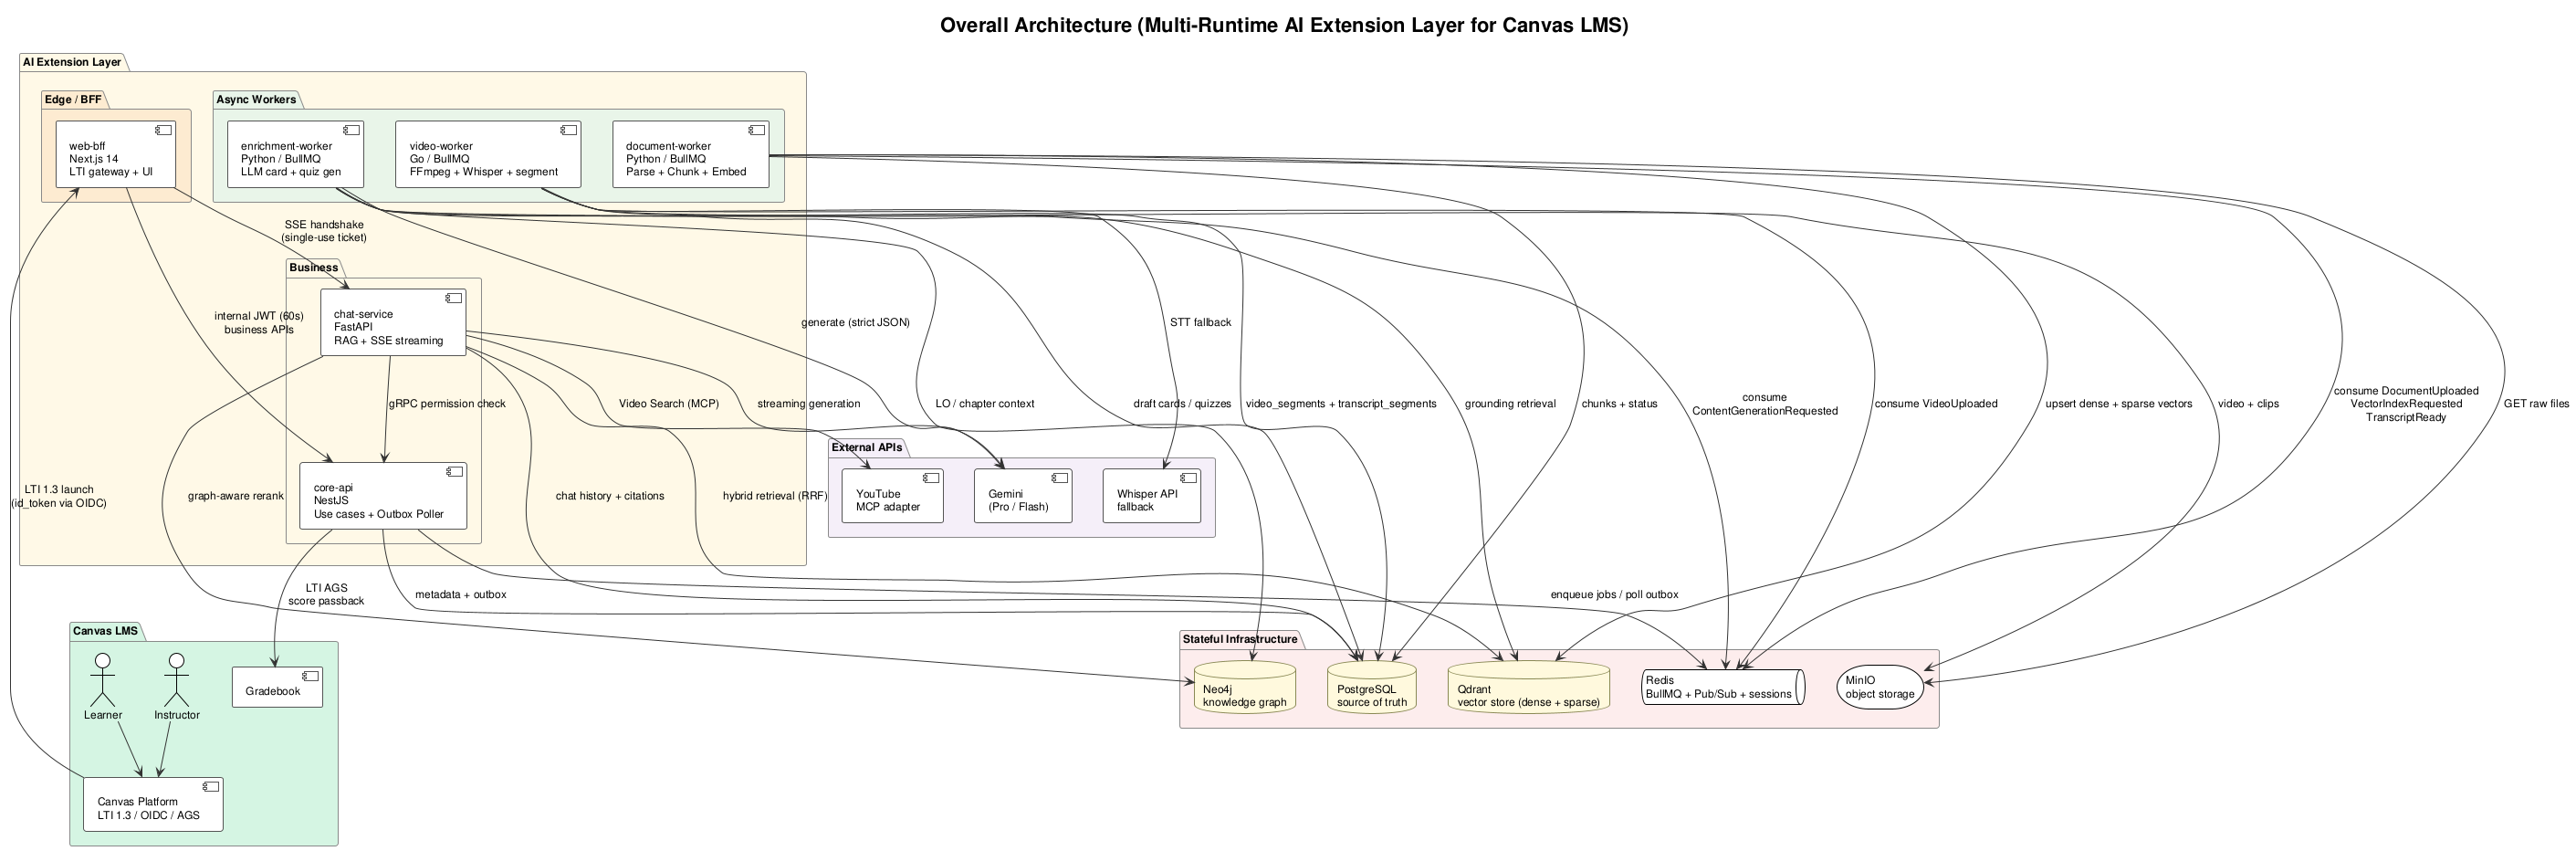
\includegraphics[width=0.95\textwidth]{diagrams/arch_overview.png}
    \caption{Overview of the multi-runtime system architecture.}
    \label{fig:arch-overview-lvtn}
\end{figure}

\subsection{AI Extension Layer Architecture}

The system is not a self-built LMS; it is an \textbf{AI Extension Layer}
attached to Canvas LMS through LTI 1.3. This approach:

\begin{itemize}
    \item reuses Canvas features for course management, users, roles, and
          gradebook;
    \item concentrates development effort on the AI layer:
          Micro-Content generation, RAG, curriculum-aware quiz, and video
          pipeline;
    \item reduces deployment risk because the institution keeps its
          existing LMS workflow and only adds an external LTI Tool.
\end{itemize}

Learners and instructors access the system through an activity embedded in
a Canvas course. When they click the activity, Canvas initiates an LTI
launch to \texttt{web-bff}; the system authenticates the launch and routes
the user to the interface corresponding to their role.

\subsection{Microservice Architecture}

The system is decomposed into \textbf{six independent Physical Runtimes}
to support horizontal scalability, dynamic scaling, and fault isolation.

It is necessary to distinguish \textbf{Physical Runtime} from
\textbf{Logical Service/Module}. The system has \textbf{six physical
runtimes} that run independently, as shown in Table~\ref{tab:runtimes}.
From the business-design perspective, however, the system contains
\textbf{nine logical services}. Each logical service is developed as an
independent module and embedded into the corresponding physical runtime
according to computational resources and communication density. This
optimizes operating cost and reduces infrastructure complexity.

\begin{table}[H]
    \centering
    \caption{Main Physical Runtimes in the system.}
    \label{tab:runtimes}
    \begin{tabular}{|p{4.4cm}|p{3cm}|p{6.6cm}|}
        \hline
        \textbf{Physical runtime} & \textbf{Technology stack} & \textbf{Role and responsibility} \\
        \hline
        \texttt{web-bff}
            & Next.js, TypeScript
            & LTI Gateway, browser BFF, instructor and learner UI. \\
        \hline
        \texttt{core-api}
            & NestJS, TypeScript
            & Main business logic, metadata, authorization, Outbox Poller daemon. \\
        \hline
        \texttt{chat-service}
            & Python FastAPI
            & Realtime AI Tutor, RAG retrieval, Video Search adapter (Internal/YouTube MCP), and SSE streaming response. \\
        \hline
        \texttt{document-worker}
            & Python, BullMQ
            & Document parsing (PDF/OCR), chunking, text embedding. \\
        \hline
        \texttt{enrichment-worker}
            & Python, BullMQ
            & Calls LLM APIs to generate lesson cards, key concepts, and quizzes. \\
        \hline
        \texttt{video-worker}
            & Go, FFmpeg
            & Audio extraction, Speech-to-Text, video segmentation. \\
        \hline
    \end{tabular}
\end{table}

Six principles apply throughout the architecture:

\begin{enumerate}
    \item \textbf{API requests do not process heavy tasks:} PDF parsing,
          transcription, embedding, and LLM batches are pushed to workers
          through a message broker, avoiding HTTP/gRPC timeouts.
    \item \textbf{Realtime chat does not go through a queue:}
          \texttt{chat-service} handles chat synchronously through SSE so
          tokens can be streamed in real time.
    \item \textbf{PostgreSQL is the only source of truth:} Qdrant (Vector)
          and Neo4j (Graph) are derived stores. Qdrant upserts are
          performed inside the same worker job that writes chunks to
          PostgreSQL, so no Outbox is needed for the vector store. Neo4j,
          on the other hand, cannot participate in a PostgreSQL
          transaction and therefore uses the Outbox pattern: every
          data-changing action is recorded transactionally in
          PostgreSQL together with an \texttt{outbox\_events} row, and an
          Outbox Poller daemon in \texttt{core-api} reads these events
          and dispatches graph-sync jobs through BullMQ. This keeps
          high transactional integrity while only paying the Outbox cost
          where it is actually required.
    \item \textbf{Asynchronous broker communication removes direct
          coupling:} Workers primarily exchange results through events on
          Redis/BullMQ. Direct network calls (gRPC or HTTP) between workers
          are minimized to avoid network coupling and temporal coupling.
    \item \textbf{Time-ordered primary keys (UUIDv7):} high-write,
          large-data tables such as \texttt{chunks},
          \texttt{learning\_events}, \texttt{chat\_messages}, and
          \texttt{outbox\_events} use UUIDv7 instead of traditional UUIDv4.
          The embedded timestamp makes PostgreSQL B-Tree indexes insert in
          near-sequential order, reducing B-Tree index fragmentation and
          improving bulk-write throughput.
    \item \textbf{Soft Delete and Consumer Idempotency:} the system uses
          Soft Delete (\texttt{deleted\_at}) at the relational database
          layer for root entities, preventing cascading deletion and data
          loss. Workers for Neo4j and Qdrant are idempotent consumers:
          Qdrant upsert uses each chunk's unique UUID, while Neo4j uses
          Cypher \texttt{MERGE}, ensuring that reprocessing an event does
          not create duplicate or orphaned data.
\end{enumerate}

\subsection{Layered Architecture}

Each AI/business runtime is organized using the Hexagonal layered
structure shown in Figure~\ref{fig:hexagonal-lvtn}, with four main
layers:

\begin{itemize}
    \item \textbf{Delivery (Primary Adapter):} HTTP API (FastAPI/NestJS),
          gRPC server, BullMQ worker, SSE handler.
    \item \textbf{Application:} use case orchestration, DTO mapping,
          transaction control.
    \item \textbf{Domain:} entity, value object, Port interface, business
          rule. This layer does not depend on frameworks.
    \item \textbf{Infrastructure (Secondary Adapter):} PostgreSQL adapter,
          Qdrant client, Neo4j driver, MinIO client, LLM/embedding client.
\end{itemize}

\begin{figure}[H]
    \centering
    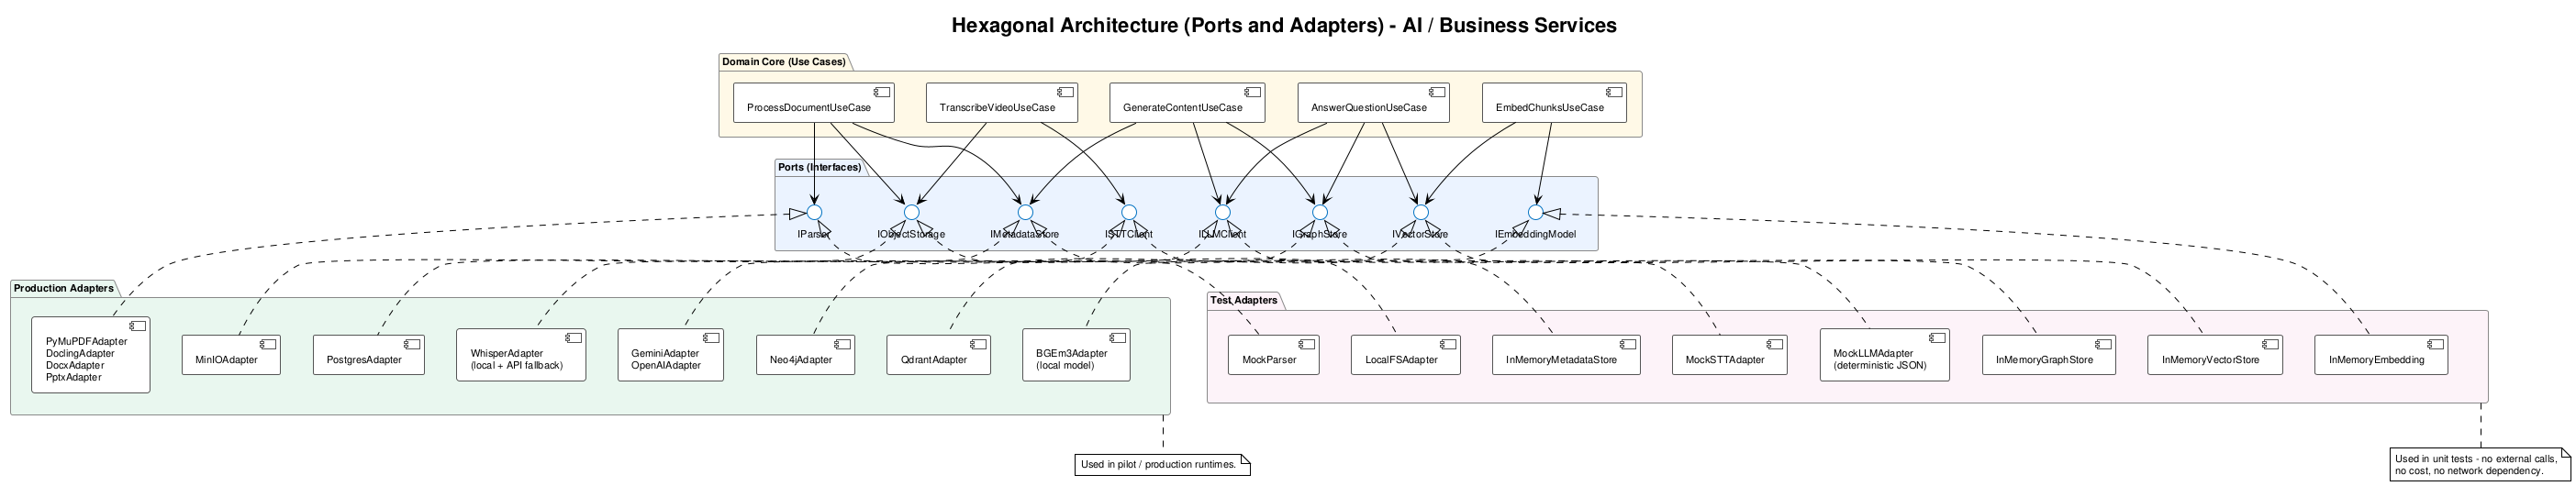
\includegraphics[width=0.95\textwidth]{diagrams/arch_hexagonal.png}
    \caption{Hexagonal layered architecture in AI/business services.}
    \label{fig:hexagonal-lvtn}
\end{figure}

\subsection{Architectural Design Philosophy}

\subsubsection*{a. Domain-Driven Design}

The Domain Model is designed around clear bounded contexts:
\textbf{Content Authoring} (document, chunk, card, quiz),
\textbf{Curriculum} (course, chapter, learning outcome, assessment),
\textbf{Video Library} (video, segment, transcript), and
\textbf{Learning} (student attempt, mastery, progress). Each context has
its own entities, repositories, and use cases. Communication between
contexts is performed through events or explicit APIs; one context does
not directly access another context's internal entities.

\subsubsection*{b. Hexagonal Architecture}

The Domain layer defines Port interfaces (abstract base classes) for
every external dependency: \texttt{IParser}, \texttt{IEmbeddingModel},
\texttt{IVectorStore}, \texttt{IMetadataStore}, \texttt{IGraphStore},
\texttt{IObjectStorage}, and \texttt{ILLMClient}. Adapters implement
these Ports using concrete technologies. When the LLM provider (Gemini
$\to$ OpenAI) or vector store (Qdrant $\to$ Pinecone) changes, only the
Adapter changes; Domain and Application remain untouched. Dependency
injection through a Container wires Adapters into Use Cases at bootstrap,
not at runtime.

\subsubsection*{c. Event-driven Architecture}

Long-running tasks (parse, chunk, embed, transcribe, generate) are
decoupled from direct request/response through the message broker.
\texttt{core-api} only publishes events/commands to the broker and
immediately returns a document/video ID. Workers consume events and, after
processing, publish new events such as \texttt{DocumentParsed},
\texttt{TranscriptReady}, and \texttt{ContentDraftGenerated}. Pipeline
state is tracked through state machines, allowing each step to retry
independently.

\section{Functional Subsystem Design}

Section 4.1.2 established the six physical runtimes of the system. On top
of these runtimes, business capabilities are decomposed into nine logical
subsystems with independent responsibility boundaries. Separating
``functional subsystem'' from ``physical runtime'' allows packaging
boundaries to be rearranged when performance requirements change, for
example splitting a module into its own runtime when load increases,
without changing business logic. Table~\ref{tab:service-to-runtime}
summarizes how the nine subsystems are embedded into their corresponding
runtimes.

\begin{table}[H]
    \centering
    \caption{Mapping functional subsystems to physical runtimes.}
    \label{tab:service-to-runtime}
    \begin{tabular}{|p{4.5cm}|p{5cm}|p{4cm}|}
        \hline
        \textbf{Logical subsystem} & \textbf{Resident runtime} & \textbf{Load characteristic} \\
        \hline
        LMS Integration / LTI & \texttt{web-bff} & I/O, launch-hour peak \\
        \hline
        Document Processing & \texttt{document-worker} & CPU/RAM, bursty \\
        \hline
        AI Generation & \texttt{enrichment-worker} & LLM API I/O \\
        \hline
        Video Processing & \texttt{video-worker} & CPU/GPU, long-running \\
        \hline
        Chatbot / RAG & \texttt{chat-service} & Realtime streaming \\
        \hline
        Curriculum & \texttt{core-api} + \texttt{document-worker} & Burst during ingestion \\
        \hline
        Learning Analytics & \texttt{core-api} & Learning-event based \\
        \hline
        Observability & cross-cutting in every runtime & Continuous \\
        \hline
        Video Search & module in \texttt{chat-service} & Per question \\
        \hline
    \end{tabular}
\end{table}

Each subsystem is presented from three consistent perspectives:
(i) \textit{responsibility}, which describes the functional boundary;
(ii) \textit{runtime placement}, which explains why the subsystem is
placed in the chosen runtime instead of split or merged; and
(iii) \textit{notable design points}, which clarify key technical
decisions.

\subsection{LMS Integration and LTI}

\textbf{Responsibility.} This is the only gateway between Canvas LMS and
the whole system. The subsystem starts the LTI 1.3 session using OIDC,
verifies the \texttt{id\_token} through Canvas JWKS, and maps
\texttt{(lms\_type, lms\_sub)} to \texttt{internal\_user\_id} through
\texttt{lms\_user\_mappings}.

\textbf{Runtime placement.} It is placed in \texttt{web-bff} (Next.js)
because this gateway must receive form-POST requests from the Canvas
browser context and set the session cookie. This is a natural
responsibility of an edge runtime close to users. A separate runtime would
not offer meaningful scaling benefits, because peak load only occurs when
many learners launch the tool at the same time, while it would add one
extra network hop to every login session.

\textbf{Notable design point.} The system uses a \emph{two-layer token}
mechanism to isolate Canvas sessions from internal services. The original
session is stored in Redis (TTL 30 minutes), but every request forwarded
from \texttt{web-bff} to \texttt{core-api} carries a short-lived internal
JWT (60 seconds) signed by BFF's private key. The SSE channel, which does
not support Custom Headers in standard \texttt{EventSource}, uses a
\emph{Single-Use Ticket}: the token is placed in the handshake query
string and checked only once when opening the connection. After the
connection is accepted, the stream stays open via keep-alive and does not
depend on the initial ticket lifetime.

\subsection{Document Processing}

\textbf{Responsibility.} This subsystem transforms source files into
structured text chunks: download files from MinIO, parse PDF/DOCX/PPTX
(with OCR fallback when the text layer is poor), normalize heading/page
metadata, split chunks by heading or size, and emit
\texttt{DocumentParsed} for downstream steps.

\textbf{Runtime placement.} It is separated into its own
\texttt{document-worker} instead of being merged with the AI worker. Large
PDF parsing and chunking are CPU/RAM-bound tasks that can consume
1--2~GB RAM for a complex syllabus file. Running them together with the
LLM-calling worker, which is I/O-bound, would block the event loop and
make resource limits difficult to tune for two different workload types.

\textbf{Notable design point.} The worker is idempotent: chunks use UUIDv7
as primary keys, and all operations are upserts rather than blind inserts
when jobs retry. Parse results are committed to PostgreSQL in the same
transaction as the synchronization outbox event, ensuring that indexing
and graph sync remain consistent even if the next process is interrupted.

\subsection{AI Generation}

\textbf{Responsibility.} This subsystem generates learning artifacts such
as lesson cards, key concept cards, and quiz items from indexed text
chunks. The \texttt{TextIndexed} event only signals that source data is
ready; artifact generation is triggered by separate
\texttt{ContentGenerationRequested} events with \texttt{type=card} or
\texttt{type=quiz}. The \texttt{enrichment-worker} groups chunks by
level-2 heading or Learning Outcome, calls the LLM with strict JSON
schema, validates output, and stores artifacts in
\texttt{GENERATED\_DRAFT}.

\textbf{Runtime placement.} It is separated into the dedicated
\texttt{enrichment-worker}. Its I/O-bound nature, where each LLM call may
wait 5--30 seconds and must use exponential backoff on HTTP 429, makes
isolation from CPU-bound workers necessary. LLM-provider rate limits will
not block the document-parse pipeline, and replicas can be tuned
independently according to each queue's depth.

\textbf{Notable design point.} Every artifact stores
\texttt{source\_chunk\_ids} and, when available, \texttt{lo\_id}, so
instructors can trace its origin. There is no automatic publish
mechanism; all content must go through instructor review, described in
Section~\ref{subsec:review-publish-pipeline}.

\subsection{Video Processing}

\textbf{Responsibility.} This subsystem transforms raw video files into
timestamped transcripts and referenceable segments. The pipeline includes
audio extraction with FFmpeg, Whisper STT, segmentation based on silence
gaps and topic shifts, cutting 30--90 second clips, and storing segment
metadata in PostgreSQL.

\textbf{Runtime placement.} It is placed in \texttt{video-worker} written
in Go because the pipeline depends on many subprocesses (FFmpeg, Whisper)
and benefits from goroutine-based parallel orchestration. The container
is configured to access GPU through Docker Compose
\texttt{deploy.resources.reservations.devices}, using Nvidia CUDA Toolkit
to accelerate Whisper on long videos.

\textbf{Notable design point.} Processing a lecture video, often longer
than 60 minutes, exceeds BullMQ's default stalled-job detection threshold
(30 seconds). Therefore, the worker calls \texttt{job.progress()} every
10 seconds to confirm progress and prevent Redis broker from reclaiming
the running job and dispatching it to another instance. When complete,
the worker only publishes \texttt{TranscriptReady} through the broker;
there is no direct gRPC connection to the Python worker, keeping
cross-language communication stateless.

\subsection{Chatbot / RAG}

\textbf{Responsibility.} This subsystem answers learner questions using
Retrieval-Augmented Generation. It receives the internal JWT containing
\texttt{course\_id} and \texttt{roles}, queries Qdrant for similar chunks
with a hard course filter, enriches context with LO knowledge from Neo4j,
assembles the prompt, and streams the response through SSE.

\textbf{Runtime placement.} It is separated as \texttt{chat-service}
(FastAPI) because it is the only endpoint requiring low latency and long
streaming connections. Merging it into \texttt{core-api} would keep HTTP
connections open in a framework that is not streaming-native (NestJS),
while a separate runtime allows independent scaling by the number of
online learners.

\textbf{Notable design point.} The SSE endpoint is protected by the
Single-Use Ticket mechanism described in LMS Integration: authorization is
checked at the handshake stage and the token is not refreshed during the
stream. The retrieval pipeline uses \emph{hybrid search} (dense vector +
sparse keyword) through BGE-M3 and reranks by Reciprocal Rank Fusion
(Section~\ref{subsec:rag-pipeline}).

\subsection{Video Search}
\label{subsec:video-search-service}

\textbf{Responsibility.} This subsystem finds illustrative videos for a
learning question from two sources: the internal uploaded-video repository
(whose transcripts are indexed by \texttt{document-worker} into Qdrant)
and YouTube. Requests from the LLM or instructor are converted into
queries, sanitized, and returned as ranked video results.

\textbf{Runtime placement.} It is embedded as a module inside
\texttt{chat-service} instead of being split into a separate runtime.
Video Search load is driven by learner questions, because each question
may trigger a search, so it follows the load of \texttt{chat-service}. A
separate runtime would add a network round trip per question without
clear independent scaling benefits.

\textbf{Notable design point.} YouTube integration goes through a Model
Context Protocol (MCP) server instead of directly calling YouTube Data
API. MCP provides a standardized adapter layer, allowing the video source
to change (YouTube $\to$ Vimeo $\to$ another repository) without changing
chat logic. Input from the LLM is strictly sanitized before being sent to
MCP: special characters are removed and the query is capped at 100
characters to prevent command injection through tool-call parameters.

\subsection{Curriculum}

\textbf{Responsibility.} This subsystem extracts and manages CDIO-style
course structure from the course syllabus. It is executed through two
paths: CRUD APIs reside in \texttt{core-api} for UI queries/mutations,
while extraction runs in \texttt{document-worker} when instructors upload
the syllabus PDF.

\textbf{Runtime placement.} It is split to separate realtime API from
batch extraction. The extraction pipeline reuses the existing PDF parser
and OCR environment inside \texttt{document-worker}, avoiding duplicate
dependencies. Splitting extraction into a separate runtime is not useful
because load only spikes briefly when instructors ingest the syllabus at
the start of a semester.

\textbf{Notable design point.} The extractor uses \emph{Hybrid
Extraction}: regex and formatting heuristics classify raw data zones (LO
code, chapter, measurement table), then a low-cost LLM (Gemini 1.5 Flash)
with strict JSON schema normalizes the result into entity structures. This
approach avoids the brittleness of pure regex when the syllabus
formatting changes, while costing much less than using a strong LLM for
the whole parse task.

\subsection{Learning Analytics}

\textbf{Responsibility.} This subsystem tracks learner interactions
(card views, reading dwell time, quiz results), computes Mastery Level
for each Learning Outcome, and synchronizes grades to Canvas Gradebook
through LTI Assignment and Grade Services (AGS).

\textbf{Runtime placement.} It resides in \texttt{core-api} because
learning events are generated directly by quiz or card-view requests to
\texttt{core-api}. Processing in the same runtime avoids an extra broker
round trip for events that require immediate feedback, for example AGS
grade passback must complete before learners see scores in Canvas.
Splitting into a separate worker is only appropriate in future expansion
when computationally heavy mastery-estimation models are added.

\textbf{Notable design point.} Learning events are written to
\texttt{learning\_events} with UUIDv7 keys, which are time-ordered by
timestamp and support time-window analytics queries without index
fragmentation. AGS passback obtains an OAuth 2.0 client-credentials token
from Canvas at runtime and does not cache grades, preventing gradebook
drift when instructors manually edit grades in Canvas.

\subsection{Observability}

\textbf{Responsibility.} Unlike the eight subsystems above, Observability
is not an independent service but a set of cross-cutting mechanisms
integrated into every runtime: structured logging (JSON with
\texttt{trace\_id} and \texttt{span\_id} from OpenTelemetry), metrics
collection through Prometheus clients, and distributed tracing through
OpenTelemetry SDK using W3C Trace Context.

\textbf{Runtime placement.} There is no dedicated runtime for this
subsystem. The \texttt{pino} library (TypeScript) or \texttt{structlog}
(Python) is embedded in each service. The aggregation backends -- Loki for
logs, Prometheus for metrics, and Jaeger or Grafana Tempo for traces --
run as sidecar containers in the deployment stack.

\textbf{Notable design point.} Each browser request receives a
\texttt{trace\_id} (W3C Trace Context) automatically at \texttt{web-bff}
and propagates through the \texttt{traceparent} header across all layers.
For BullMQ queues, which do not automatically propagate headers, context
is serialized into the job payload and restored in the worker. This allows
complete tracing from a UI click until the worker finishes. LLM token
usage metrics are tracked separately for cost monitoring, with alerts
when consumption rate exceeds the allowed threshold.

\section{AI Pipeline Design}
\label{sec:ai-pipeline-design}

\subsection{Document Processing Pipeline}

\begin{figure}[H]
    \centering
    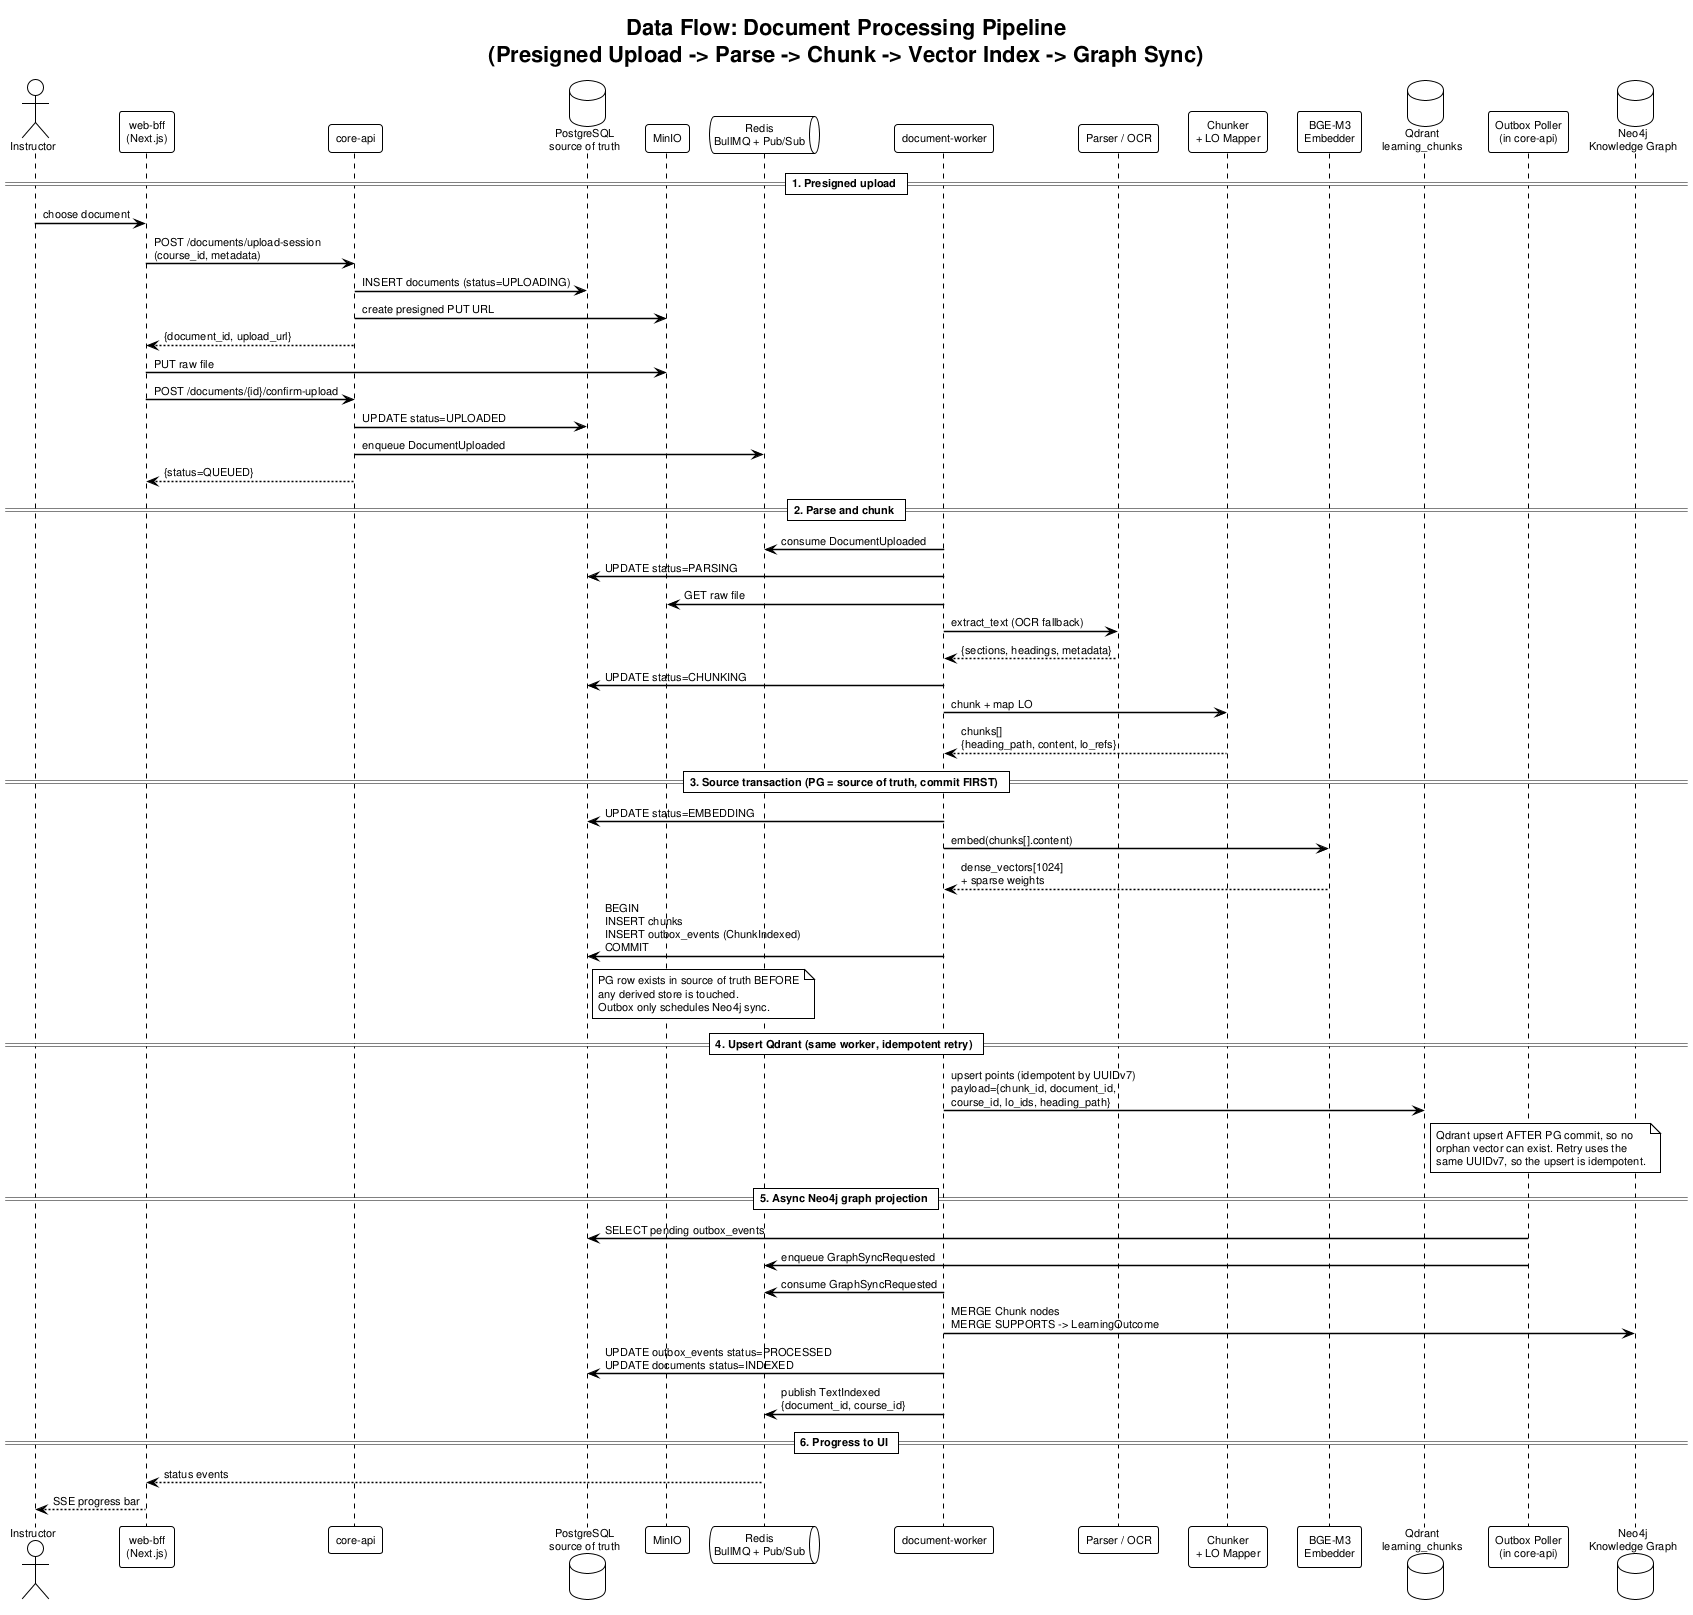
\includegraphics[width=0.95\textwidth]{diagrams/dataflow_text_pipeline.png}
    \caption{Data flow of the text/document processing pipeline.}
    \label{fig:dataflow-text}
\end{figure}

The Document Processing Pipeline is described through the data-flow
diagram in Figure~\ref{fig:dataflow-text}. It contains five main steps:
heavy tasks (parse, chunk, embed) run continuously in the same
\texttt{document-worker} job to simplify orchestration, while Outbox only
handles Knowledge Graph synchronization to Neo4j, which cannot
participate in PostgreSQL transactions:

\begin{enumerate}
    \item \textbf{Upload:} The client uploads a document to MinIO through
          a presigned URL. \texttt{core-api} records it and emits
          \texttt{DocumentUploaded} through BullMQ.
    \item \textbf{Parse and chunk:} \texttt{document-worker} consumes the
          event, downloads the file from MinIO, parses text with OCR
          fallback when needed, and splits chunks by heading or size.
    \item \textbf{Source transaction (PostgreSQL commits first):} The
          worker calls BGE-M3 to generate both dense (1024-dim) and
          sparse vectors, then commits \texttt{chunks} and the
          \texttt{outbox\_events} record (\texttt{ChunkIndexed} payload)
          to PostgreSQL in a single transaction. The PG commit happens
          \emph{before} any derived store is written, so the source of
          truth always reflects the latest state and no orphan vector can
          exist in Qdrant.
    \item \textbf{Qdrant upsert (after PG commit, idempotent):} Once the
          PG transaction succeeds, the same worker upserts the vectors
          into \texttt{learning\_chunks} with payloads
          (\texttt{course\_id}, \texttt{lo\_ids},
          \texttt{heading\_path}). Upsert is keyed by chunk UUIDv7, so a
          retry on transient failure is safe and does not create
          duplicate points.
    \item \textbf{Outbox-driven Neo4j sync:} The Outbox Poller daemon
          in \texttt{core-api} periodically scans
          \texttt{outbox\_events} and pushes graph-sync jobs to
          \texttt{document-worker}; the worker uses Cypher
          \texttt{MERGE} to create \texttt{Chunk} nodes and
          \texttt{SUPPORTS} relationships to related
          \texttt{LearningOutcome} nodes. After all chunks are indexed
          in Qdrant and projected into Neo4j, the system emits
          \texttt{TextIndexed} as the boundary event for downstream
          pipelines (Micro-Content and Quiz Generation).
    \item \textbf{UI state update:} To avoid manual reload by instructors,
          parse, chunk, and embedding steps continuously publish progress
          events through Redis Pub/Sub using BullMQ
          \texttt{job.progress()}. \texttt{web-bff} subscribes to these
          events and streams them to Next.js through a dedicated SSE
          connection. The UI updates the progress bar and document-card
          states (\texttt{UPLOADED} $\to$ \texttt{PARSING} $\to$
          \texttt{EMBEDDING} $\to$ \texttt{INDEXED}) according to the
          state machine in Section~\ref{subsec:document-pipeline-state}.
\end{enumerate}

\subsection{Video Processing Pipeline}

\begin{figure}[H]
    \centering
    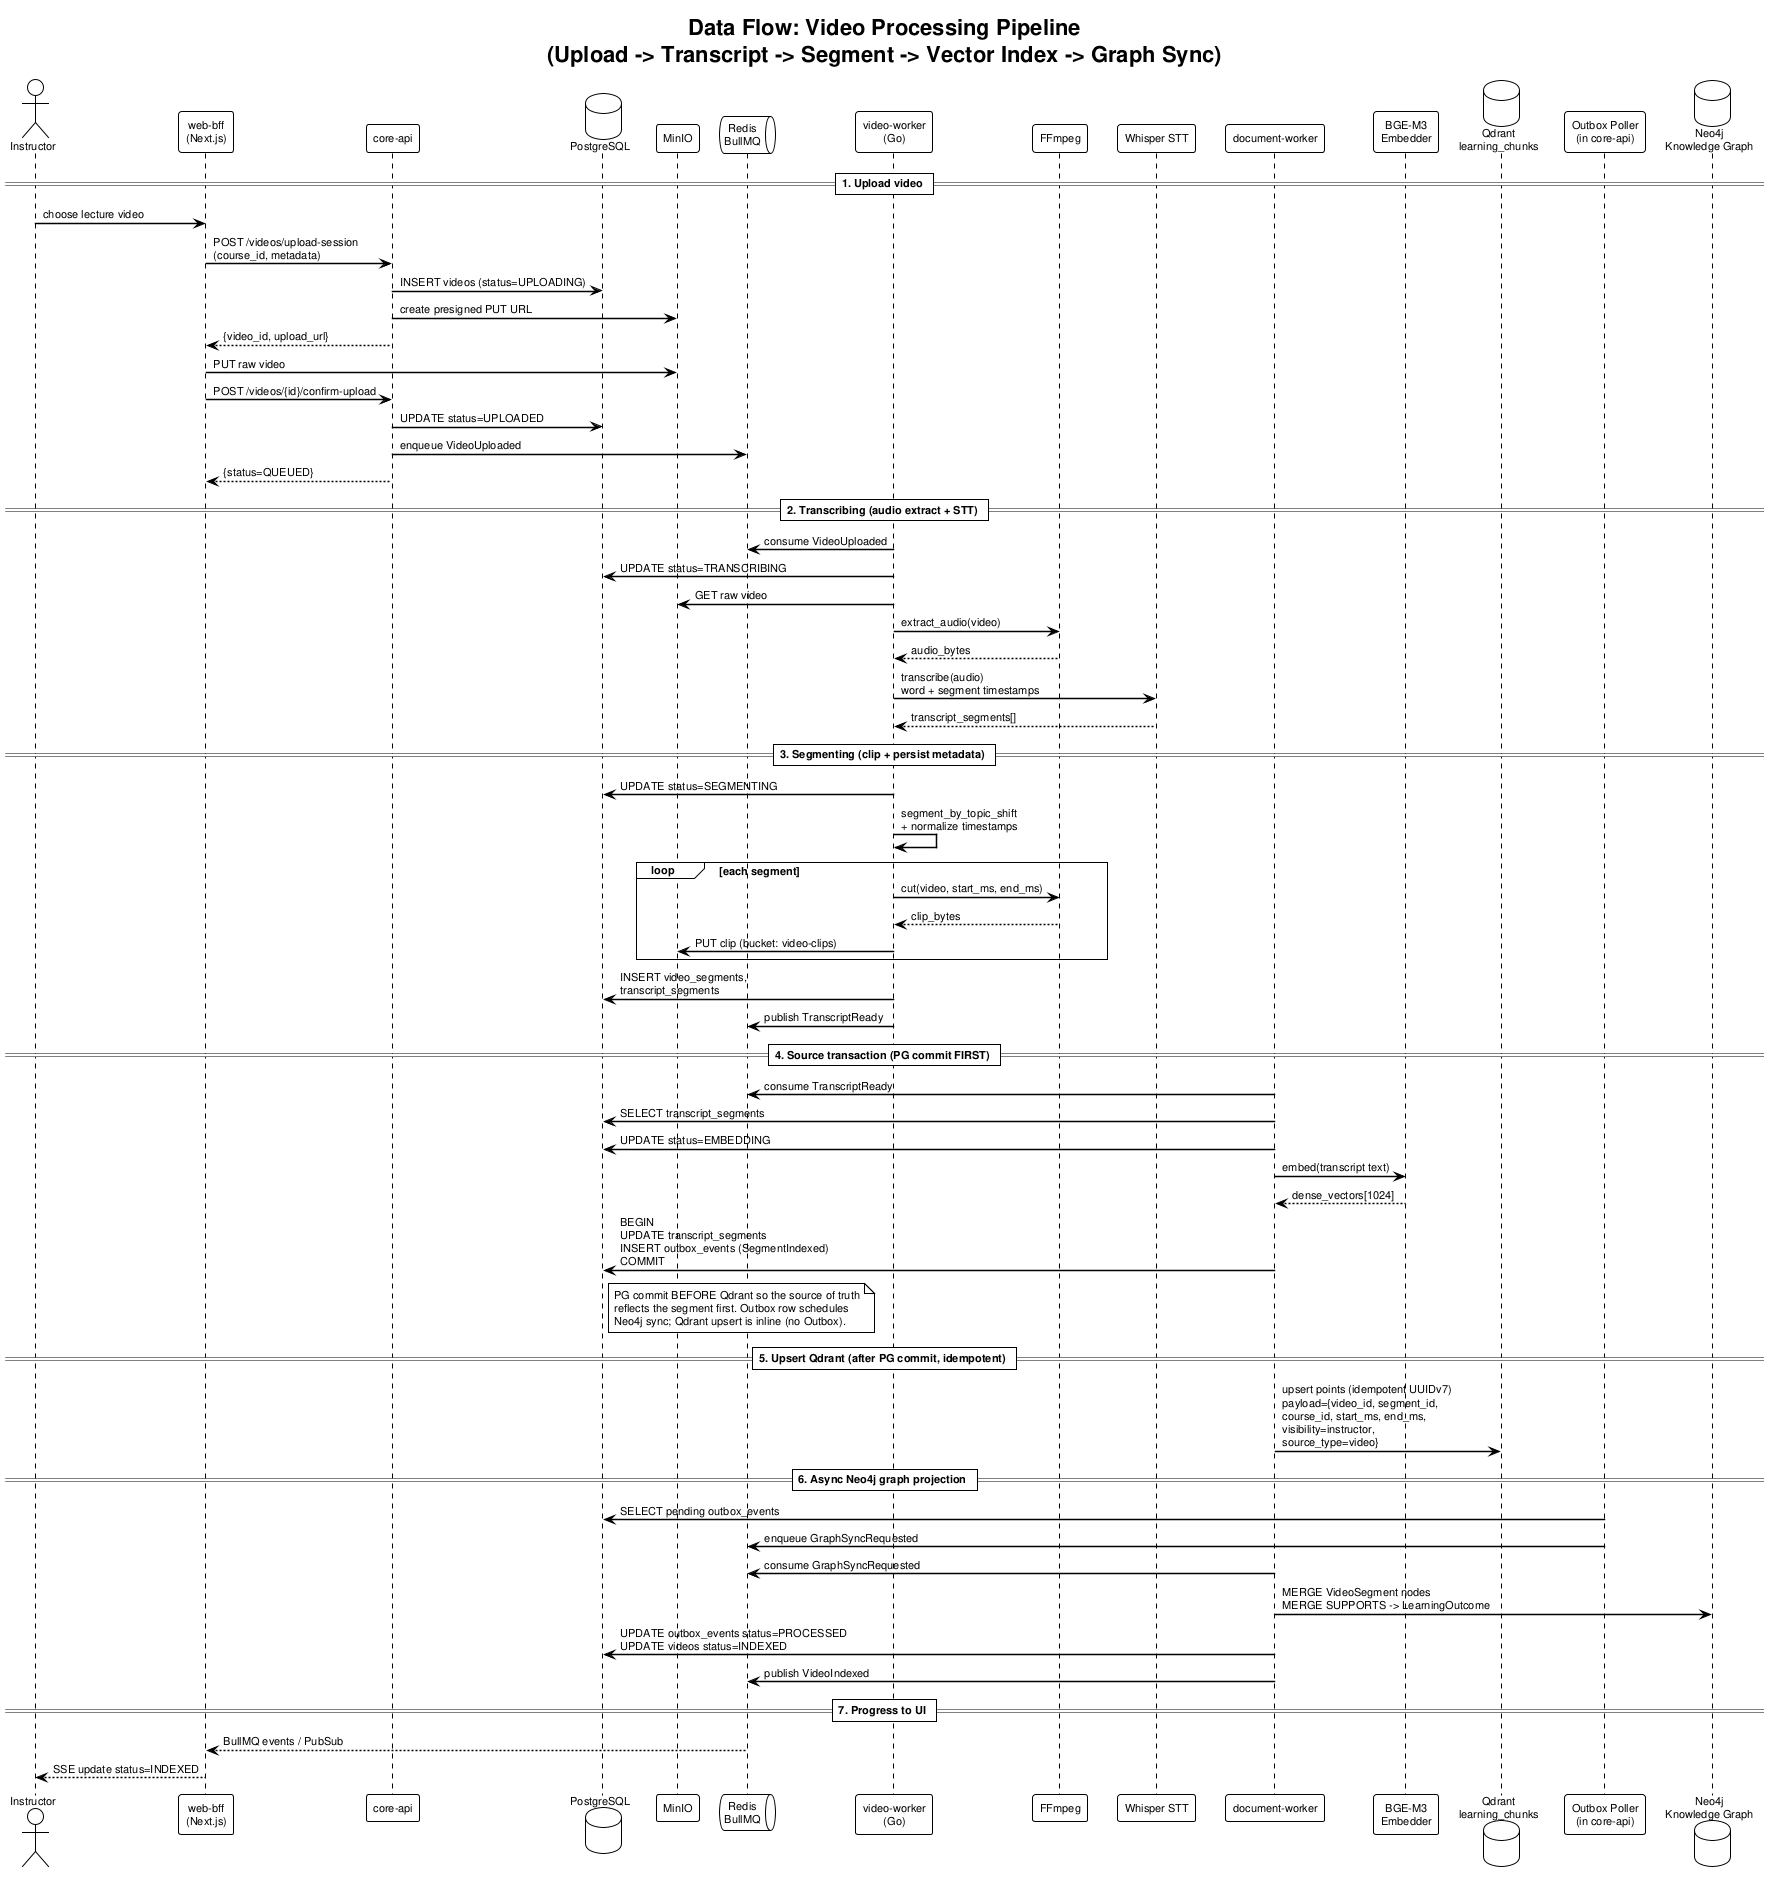
\includegraphics[width=0.95\textwidth]{diagrams/dataflow_video_pipeline.png}
    \caption{Data flow of the video processing pipeline.}
    \label{fig:dataflow-video}
\end{figure}

The video pipeline mirrors the document pipeline pattern but is split
across two runtimes: \texttt{video-worker} (Go) handles the heavy media
work (FFmpeg audio extract, Whisper STT, segment, clip) and persists
\texttt{video\_segments}/\texttt{transcript\_segments} to PostgreSQL,
then publishes \texttt{TranscriptReady}. \texttt{document-worker}
consumes that event, embeds the transcript, commits to PostgreSQL
first, upserts vectors to Qdrant after the commit, and Outbox-syncs
to Neo4j. Cross-runtime communication is exclusively through BullMQ
events on Redis -- there is no direct call between
\texttt{video-worker} and \texttt{document-worker}. See
Appendix~\ref{appendix:seq-video} for the full sequence.

\subsection{RAG Pipeline}
\label{subsec:rag-pipeline}

\begin{figure}[H]
    \centering
    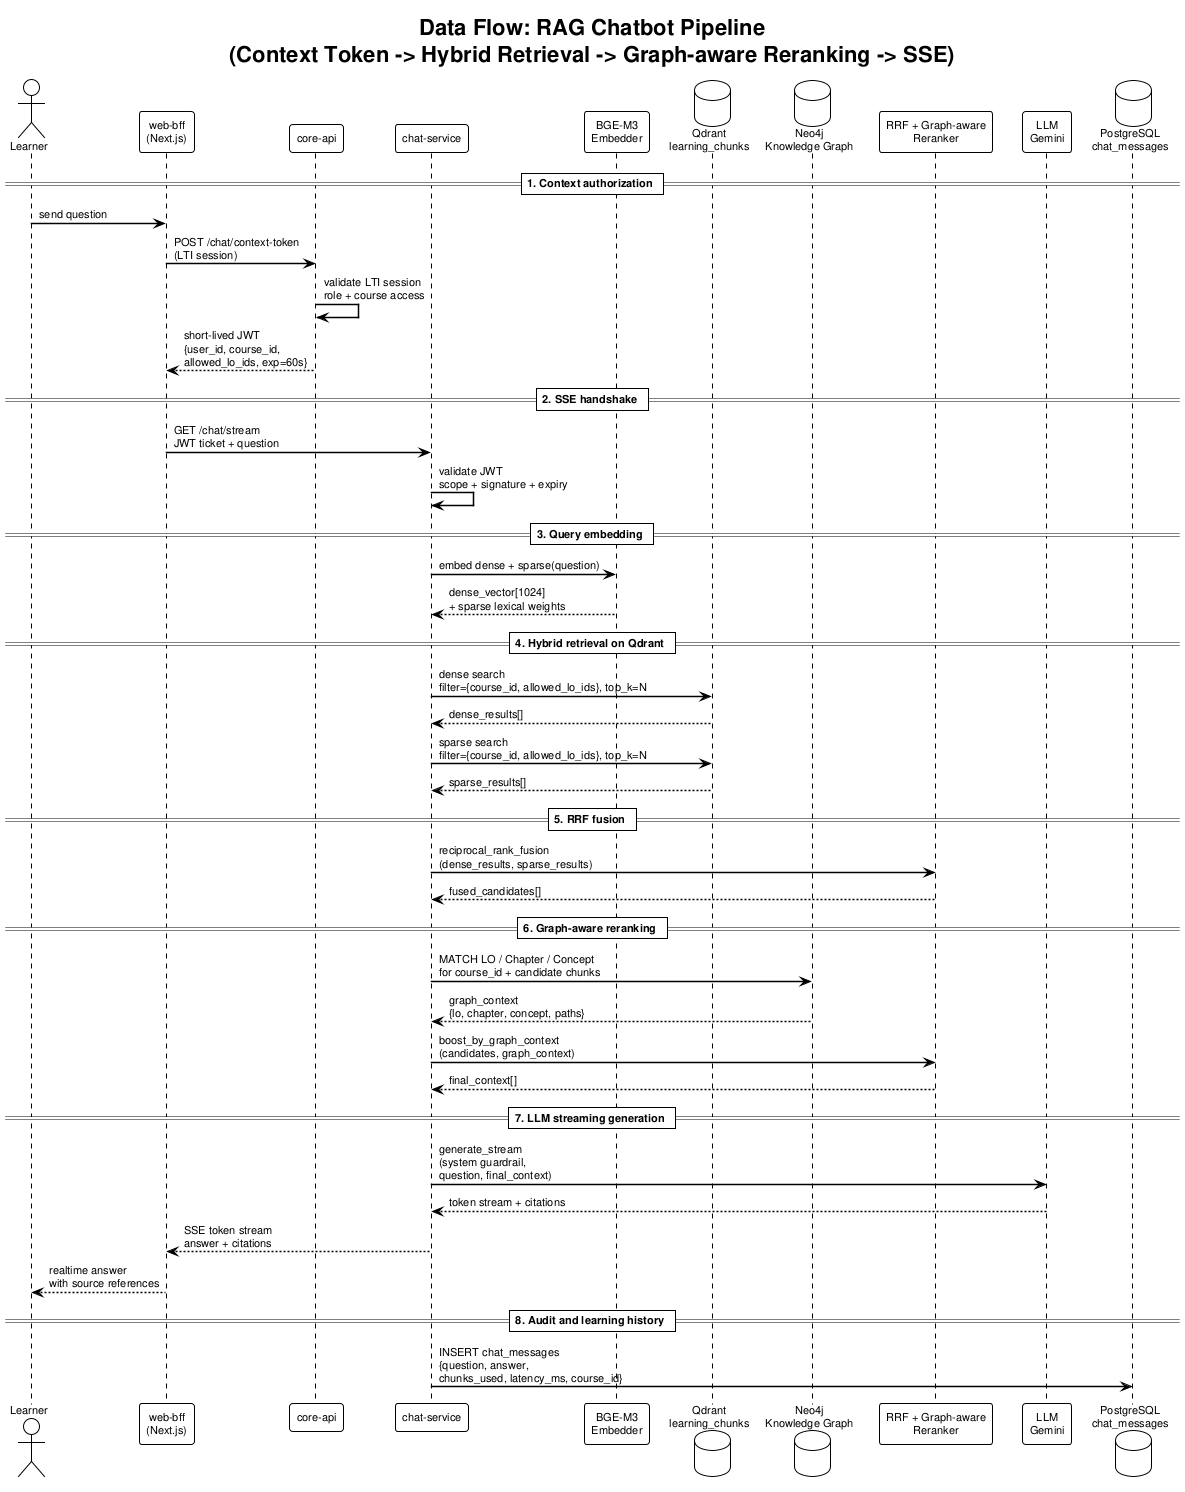
\includegraphics[width=0.95\textwidth]{diagrams/dataflow_rag_chatbot.png}
    \caption{Data flow of the RAG chatbot pipeline.}
    \label{fig:dataflow-rag}
\end{figure}

The RAG pipeline is designed as shown in Figure~\ref{fig:dataflow-rag}.
It is used for three use cases: AI Tutor Chatbot, quiz generation by LO,
and grounded lesson-summary generation. The execution flow has five main
stages:

\begin{enumerate}
    \item \textbf{Hybrid query embeddings:} When a learner sends a
          question, \texttt{chat-service} uses the multi-task
          \texttt{BGE-M3} model to generate two vector types: a dense
          vector (1024 dimensions) for deep semantics and a sparse vector
          (IDF-weighted keywords) for lexical terms specific to the query.
    \item \textbf{Hybrid retrieval on Qdrant:} The service performs a
          parallel hybrid search on Qdrant collection
          \texttt{learning\_chunks} with a mandatory hard
          \texttt{course\_id} filter for tenant isolation. Qdrant returns
          two result sets: deep semantic matches (Dense Search) and exact
          keyword matches (Sparse Search).
    \item \textbf{Score fusion and reranking (Reciprocal Rank Fusion -
          RRF):} \texttt{chat-service}, or Qdrant's orchestrator, applies
          \textbf{Reciprocal Rank Fusion (RRF)} to merge rankings from
          dense and sparse search and compute a new confidence score for
          each chunk. This fusion uses both semantic representation and
          exact matching of specialized terms/abbreviations, which pure
          semantic search often misses.
    \item \textbf{Graph-aware reranking:} The system queries Neo4j for the
          course-entity structure (LO/Chapter) and related concepts.
          Chunks lying on strong graph paths or directly linked to target
          LOs of the lesson receive a boosting multiplier and are moved
          higher in the context list.
    \item \textbf{LLM generation (streaming):} The service assembles the
          final prompt from the learner question and optimized ranked
          context, calls Gemini Pro in streaming mode, and sends response
          tokens to the learner browser in real time through SSE.
\end{enumerate}

\subsection{Micro-Content Generation Pipeline}

\begin{figure}[H]
    \centering
    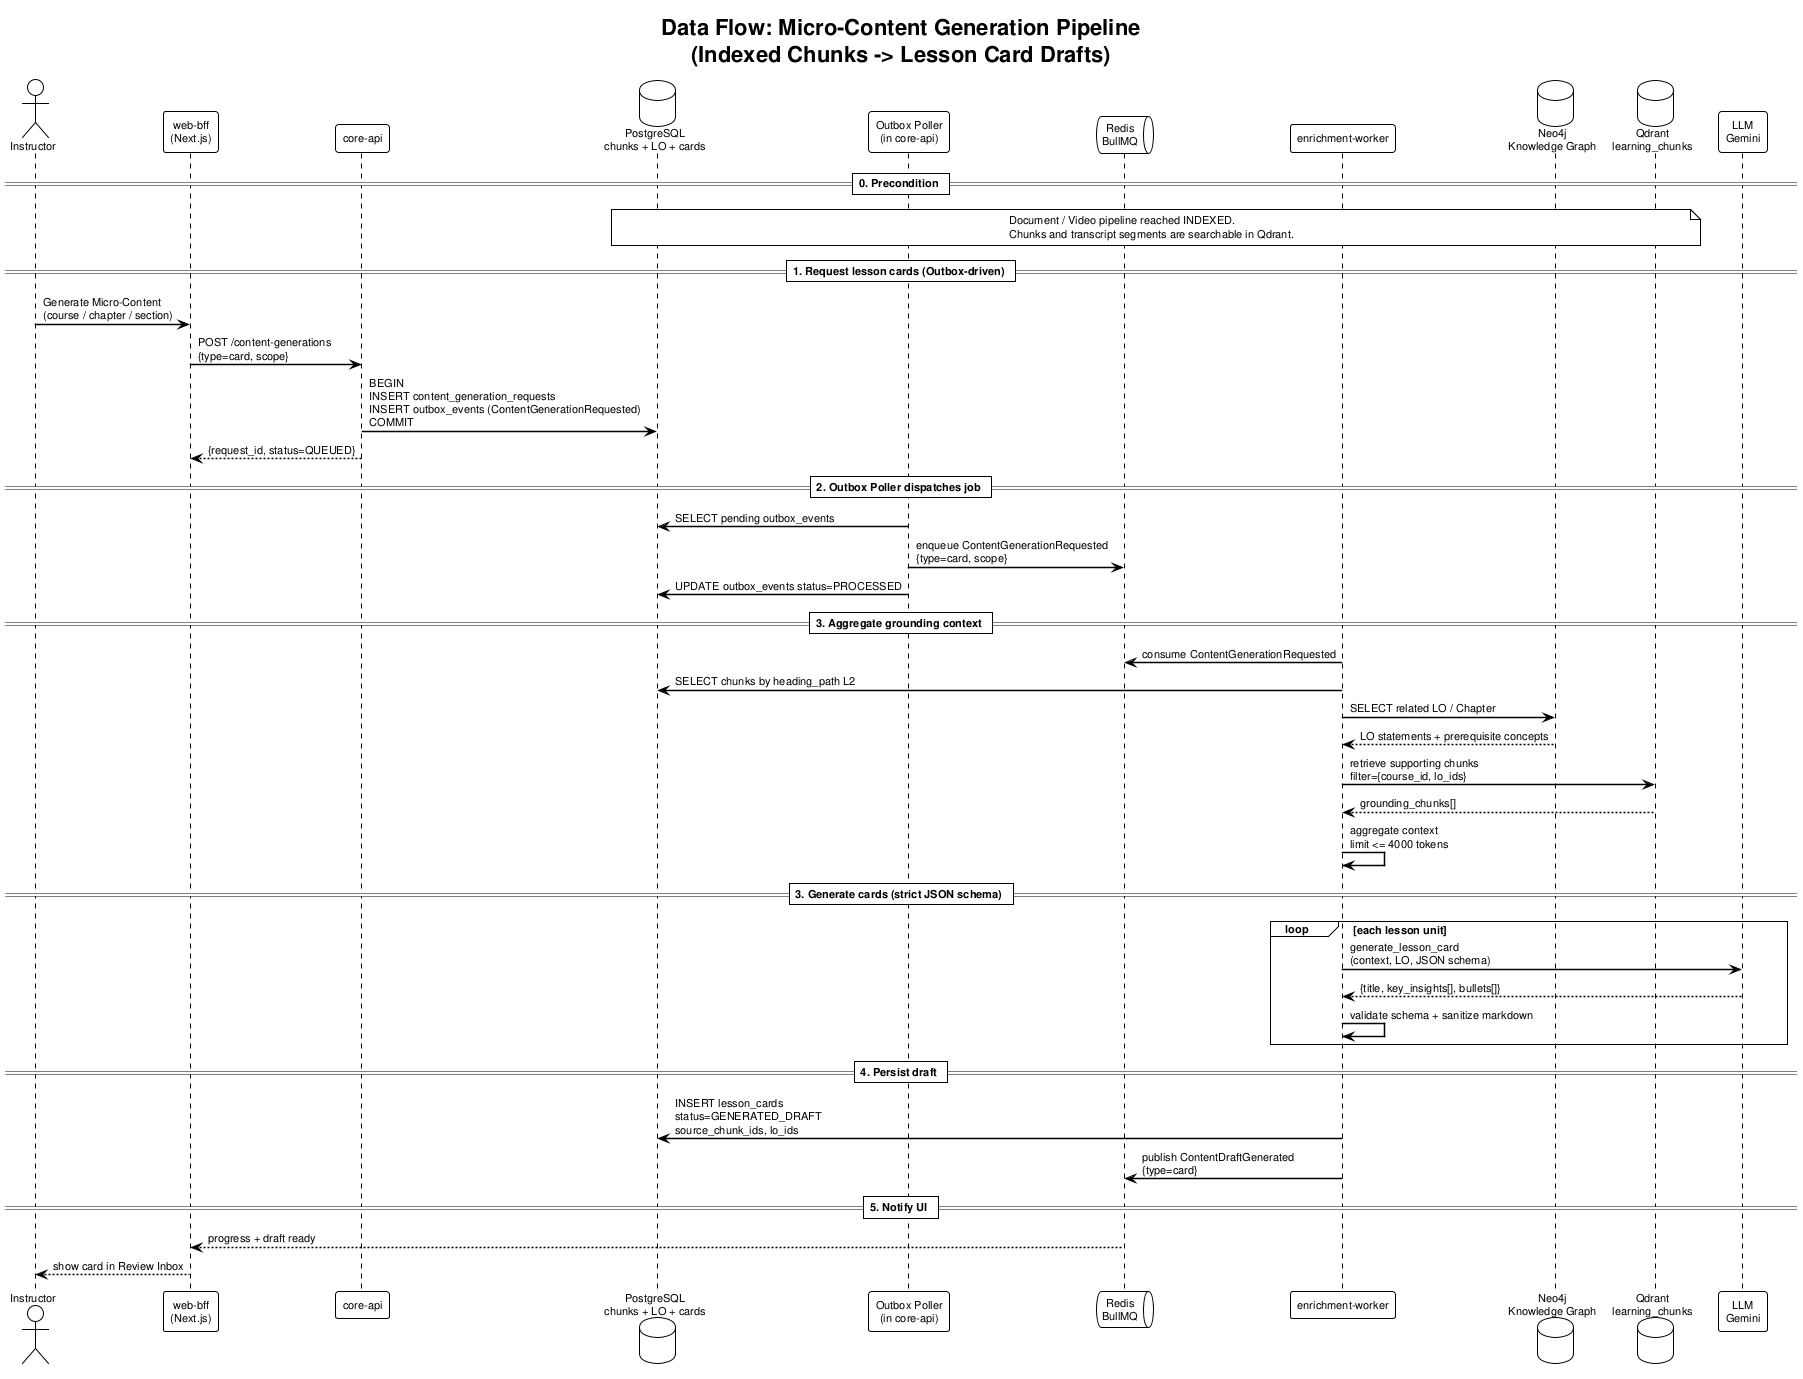
\includegraphics[width=0.95\textwidth]{diagrams/dataflow_micro_content_pipeline.png}
    \caption{Data flow of the micro-content generation pipeline.}
    \label{fig:dataflow-micro-content}
\end{figure}

\texttt{enrichment-worker} aggregates indexed chunks by level-2 heading
path (cap $\leq 4000$ tokens to control cost and avoid attention
degradation), combines them with the chapter's Learning Outcomes from
the CDIO syllabus, and asks Gemini 1.5 Pro to generate
\texttt{Lesson Cards} under a strict JSON schema (required
\texttt{title}, \texttt{key\_insights[]}, \texttt{bullets[]}). After
schema validation, drafts are persisted to \texttt{lesson\_cards} with
status \texttt{GENERATED\_DRAFT} and surfaced in the instructor review
inbox.

\subsection{Quiz Generation Pipeline}
\label{subsec:quiz-pipeline}

\begin{figure}[H]
    \centering
    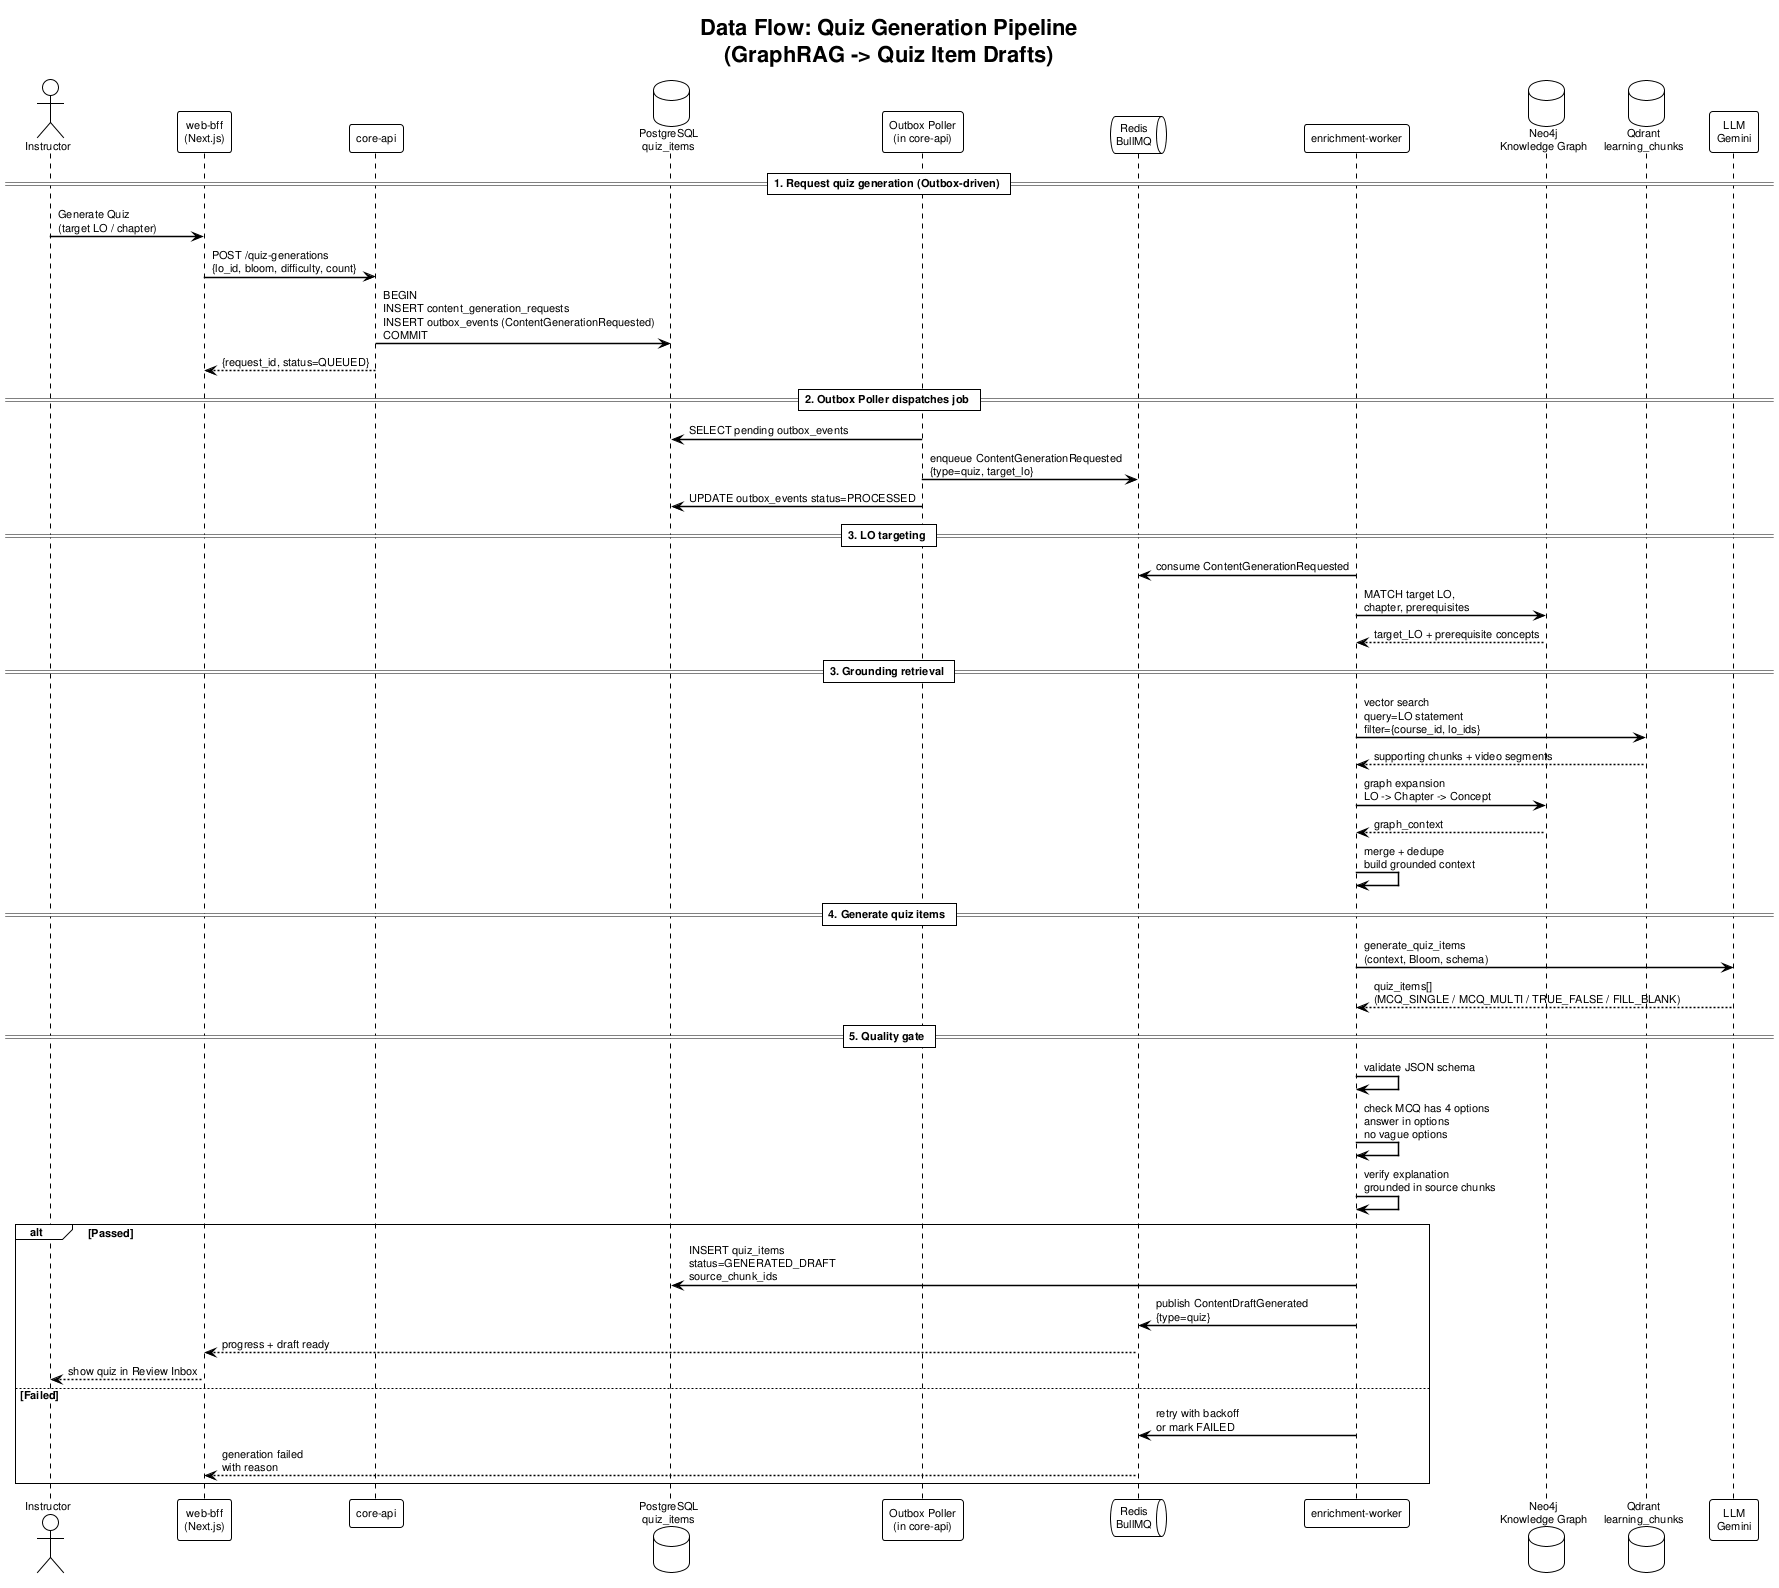
\includegraphics[width=0.95\textwidth]{diagrams/dataflow_quiz_generation_pipeline.png}
    \caption{Data flow of the quiz generation pipeline.}
    \label{fig:dataflow-quiz-generation}
\end{figure}

The multiple-choice assessment generation pipeline is designed around
GraphRAG to keep questions accurate and aligned with the university
curriculum. The execution flow contains four steps:

\begin{enumerate}
    \item \textbf{LO targeting:} When the system needs to generate a quiz
          set for a chapter, it queries Neo4j to identify all directly
          related \texttt{Learning Outcomes} and prerequisite concepts.
    \item \textbf{Grounding retrieval:} Based on the selected LO list, the
          system performs dense vector search on Qdrant to extract
          document chunks and video segments containing actual taught
          knowledge. Graph context from Neo4j and text context from Qdrant
          are integrated into the prompt to provide solid grounding for
          the LLM.
    \item \textbf{Multi-level Bloom assessment generation:} The LLM API
          call is configured with \texttt{system\_instruction} that
          strictly controls question design. The system requests the four
          question types defined in the schema --
          \texttt{MCQ\_SINGLE}, \texttt{MCQ\_MULTI},
          \texttt{TRUE\_FALSE}, and \texttt{FILL\_BLANK} -- distributed
          across Bloom cognitive levels (Remember, Understand, Apply,
          Analyze).
    \item \textbf{Quality and schema validation:} The worker runs
          automatic checks to ensure MCQs have exactly 4 choices, contain
          no ambiguous options such as ``All of the above'', have a
          correct answer that exactly matches one option, and include an
          \texttt{explanation} grounded in the raw text. Valid data is
          recorded in \texttt{quiz\_items} as
          \texttt{GENERATED\_DRAFT}.
\end{enumerate}

\subsection{Review and Publish Pipeline}
\label{subsec:review-publish-pipeline}

\begin{figure}[H]
    \centering
    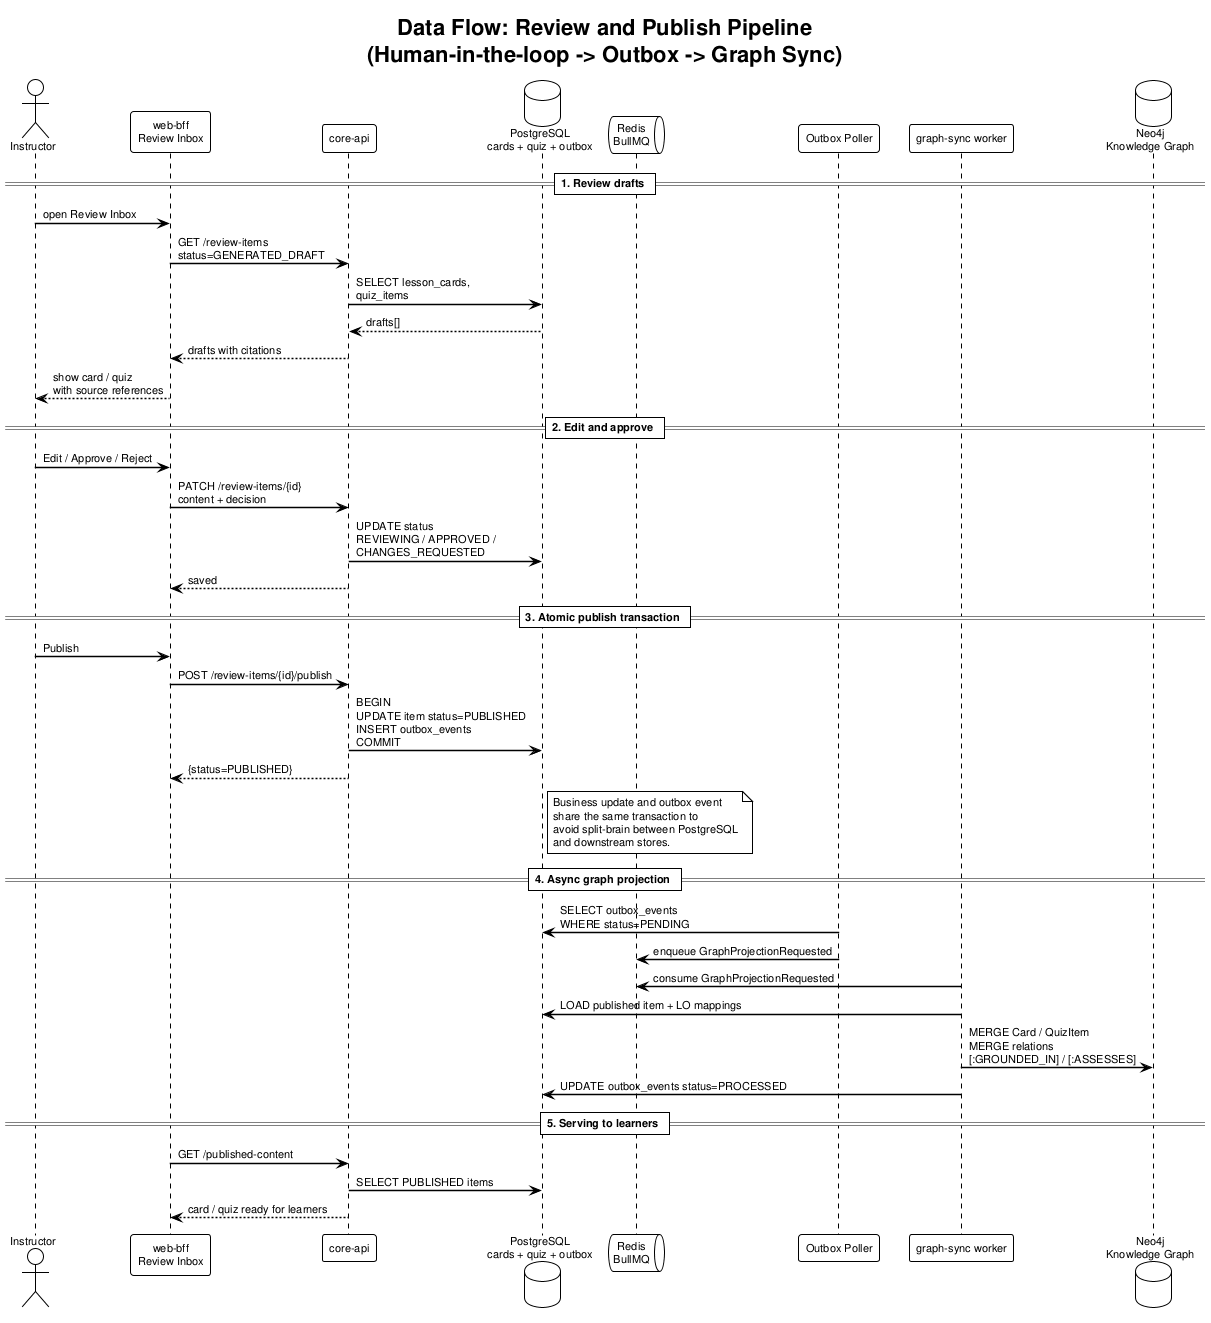
\includegraphics[width=0.95\textwidth]{diagrams/dataflow_review_publish_pipeline.png}
    \caption{Data flow of the review and publish pipeline.}
    \label{fig:dataflow-review-publish}
\end{figure}

The Human-in-the-Loop review pipeline guarantees that no AI-generated
content reaches learners without instructor approval, and that the
graph stays eventually consistent with the source of truth. When the
instructor clicks ``Publish'', \texttt{core-api} runs a single
PostgreSQL transaction that flips the row from
\texttt{GENERATED\_DRAFT} to \texttt{PUBLISHED} \emph{and} writes an
\texttt{outbox\_events} row (e.g.\ \texttt{CardPublishedEvent}) --
atomicity rules out the split-brain case where content is published
but graph sync is lost. The Outbox Poller daemon in \texttt{core-api}
later picks the event up, enqueues a BullMQ job, and a worker MERGEs
the matching \texttt{Card} or \texttt{QuizItem} node into Neo4j with
the appropriate \texttt{-[:EXPLAINS]->} or \texttt{-[:ASSESSES]->}
edge to its \texttt{LearningOutcome}.

The document deletion flow is operational rather than part of the core
AI defense argument. Its idempotent cleanup saga, which removes derived
artifacts across PostgreSQL, Qdrant, Neo4j, MinIO, and Redis cache, is
therefore provided in Appendix~\ref{appendix:delete-saga}.

\section{Database Design}
\label{sec:database-design}

\begin{figure}[H]
    \centering
    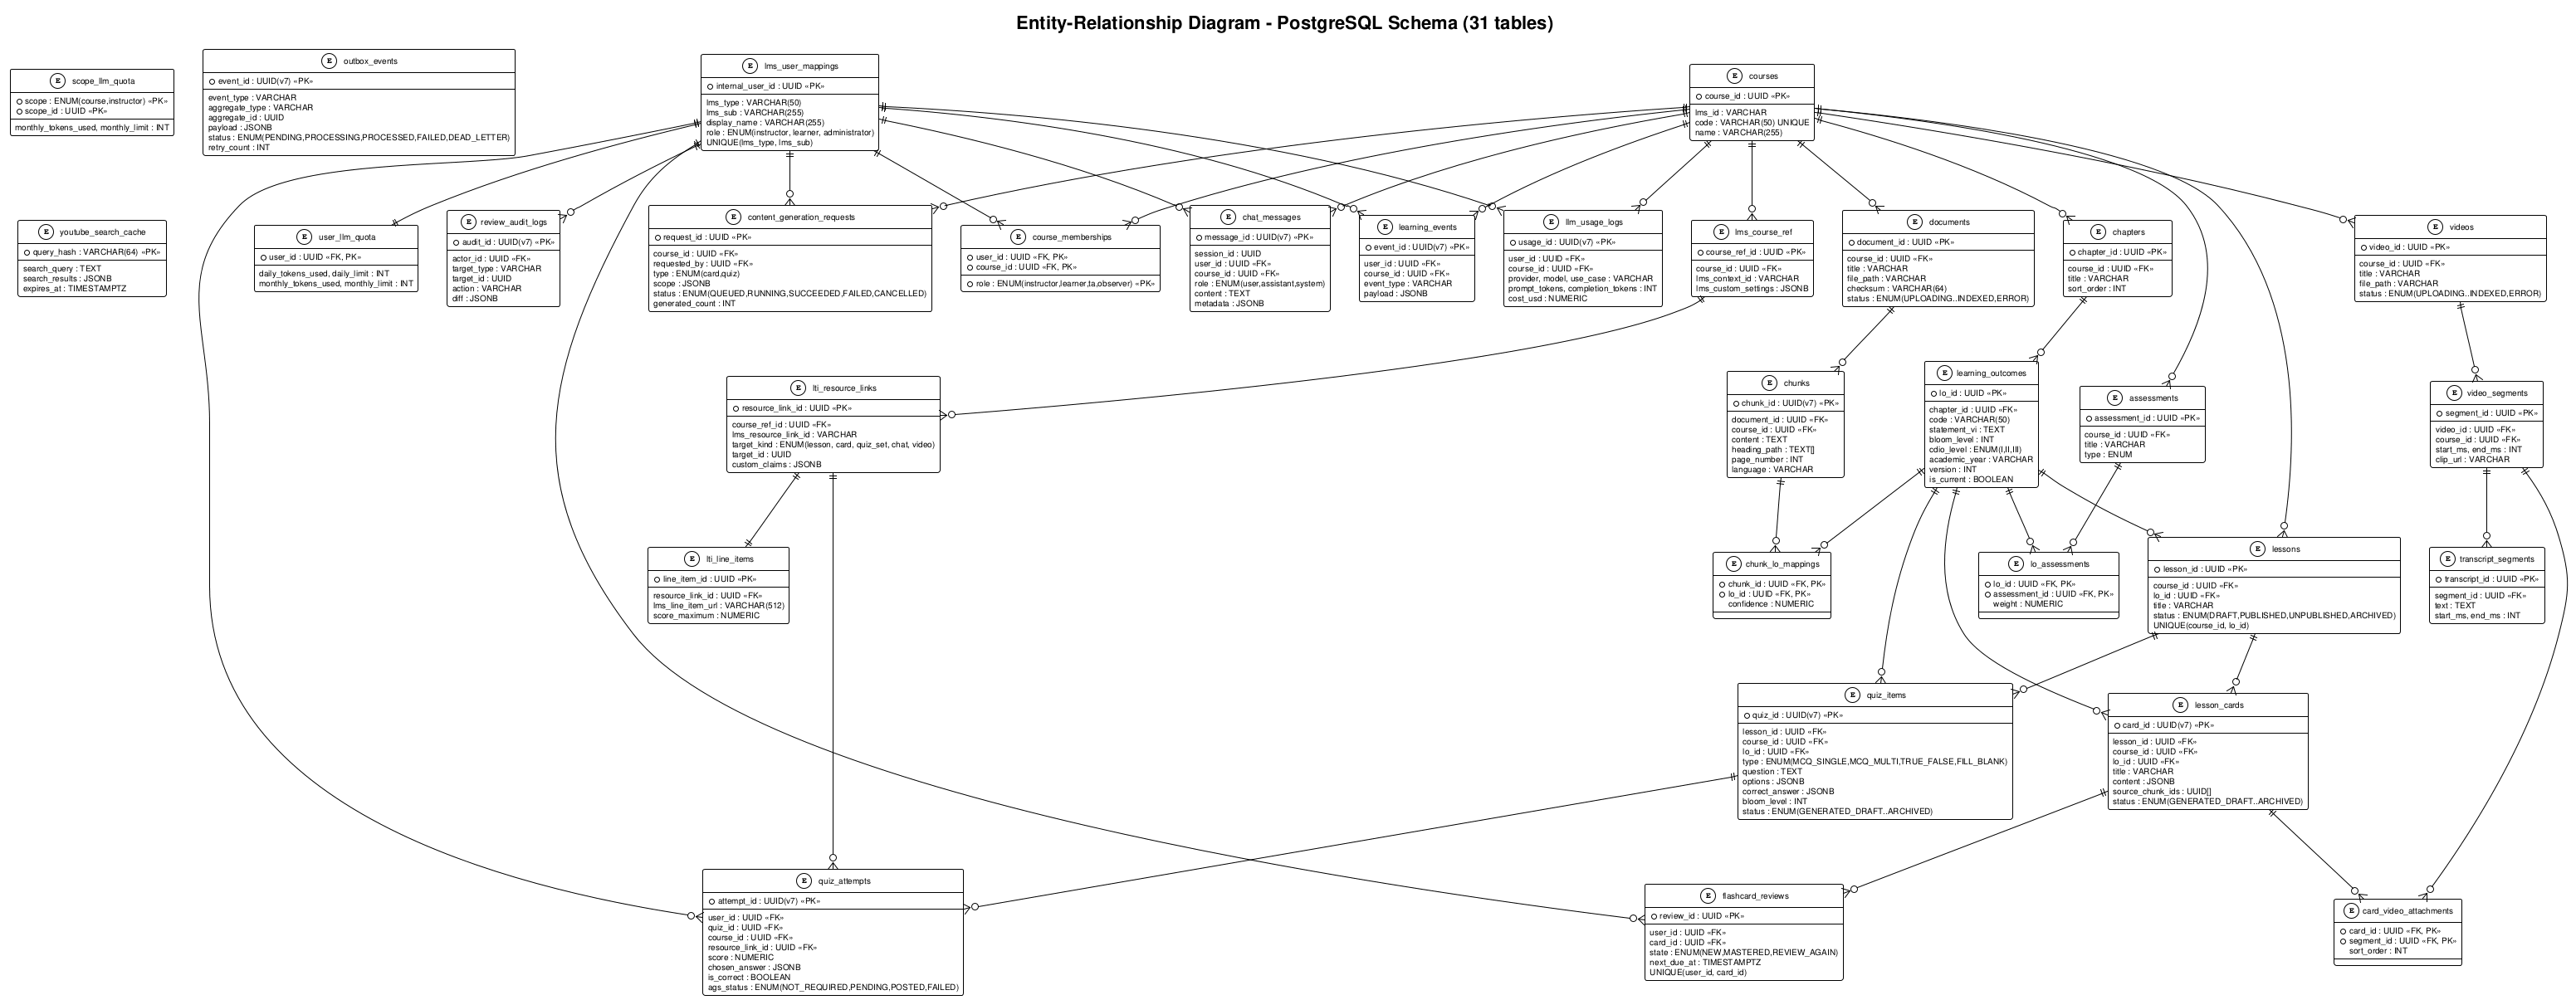
\includegraphics[width=0.95\textwidth,height=0.78\textheight,keepaspectratio]{diagrams/er_diagram.png}
    \caption{Overall ER diagram of PostgreSQL.}
    \label{fig:er-lvtn}
\end{figure}

\subsection{PostgreSQL Schema}
\label{subsec:postgres-schema}

PostgreSQL is the source of truth for all business data. The core schema
is divided into seven logical subsystems with a total of \textbf{31 core
tables} covering identity / LTI integration, ingestion, generated
content, analytics, cost tracking, and async dispatch. The implementation
adds two extension tables, \texttt{concepts} and
\texttt{chunk\_concepts}, to persist deterministic concept tags generated
by the Python pipeline. The full DDL is listed in
Appendix~\ref{appendix:db-schema}; this section summarizes the overall
structure.

\begin{table}[H]
    \centering
    \caption{Seven logical subsystems in PostgreSQL (31 core tables, plus 2 concept-tag extension tables).}
    \label{tab:postgres-tables}
    \begin{tabular}{|p{4cm}|p{9.5cm}|}
        \hline
        \textbf{Subsystem} & \textbf{Main tables} \\
        \hline
        1. LMS Integration
            & \texttt{lms\_user\_mappings}, \texttt{courses},
              \texttt{lms\_course\_ref}, \texttt{lti\_resource\_links},
              \texttt{lti\_line\_items}, \texttt{course\_memberships} \\
        \hline
        2. Curriculum (CDIO)
            & \texttt{chapters}, \texttt{learning\_outcomes},
              \texttt{assessments}, \texttt{lo\_assessments} \\
        \hline
        3. Document Ingestion
            & \texttt{documents}, \texttt{chunks},
              \texttt{chunk\_lo\_mappings}; implementation extension:
              \texttt{concepts}, \texttt{chunk\_concepts} \\
        \hline
        4. Video Pipeline
            & \texttt{videos}, \texttt{video\_segments},
              \texttt{transcript\_segments} \\
        \hline
        5. Generated Content
            & \texttt{lessons}, \texttt{lesson\_cards},
              \texttt{card\_video\_attachments}, \texttt{quiz\_items},
              \texttt{flashcard\_reviews} \\
        \hline
        6. Analytics \& Audit
            & \texttt{quiz\_attempts}, \texttt{chat\_messages},
              \texttt{learning\_events}, \texttt{review\_audit\_logs},
              \texttt{llm\_usage\_logs}, \texttt{user\_llm\_quota},
              \texttt{scope\_llm\_quota} \\
        \hline
        7. Async / Requests / Cache
            & \texttt{content\_generation\_requests},
              \texttt{outbox\_events}, \texttt{youtube\_search\_cache} \\
        \hline
    \end{tabular}
\end{table}

Key implementation notes such as LO versioning, denormalized
\texttt{course\_id}, UUIDv7 keys, content-review status constraints,
outbox indexes, and authentication delegation are kept with the schema
reference in Appendix~\ref{appendix:db-schema}.

\subsection{Qdrant Vector Schema}
\label{subsec:qdrant-vector-schema}

Qdrant stores vector embeddings for document chunks and video transcript
segments. In the MVP, a single collection \texttt{learning\_chunks} is
used, with \texttt{source\_type} distinguishing data sources. In
production, it can be split into \texttt{document\_chunks} and
\texttt{video\_segments} if optimization is needed.

\textbf{Named Vectors.} To support the \emph{Hybrid Retrieval + RRF}
pipeline described in Section~\ref{subsec:rag-pipeline}, the collection
is initialized with
two parallel vectors on the same data point:

\begin{itemize}
    \item \texttt{dense} (1024 dimensions, Cosine distance): encodes deep
          semantics, generated by the dense output of BGE-M3.
    \item \texttt{sparse} (sparse vector, IDF/BM25-style weighting):
          encodes lexical keywords, generated by the sparse output of
          BGE-M3.
\end{itemize}

\textbf{Quantization.} Dense vectors use \texttt{Scalar} (int8)
quantization with \texttt{available\_on\_ram} to reduce in-memory usage
by about four times compared with raw float32, which is especially
important on RAM-limited VPS deployment. Sparse vectors are already mostly
empty and do not need quantization.

\textbf{Payload schema and mandatory filter.} Each point carries complete
metadata for \emph{Payload Hard Filtering} before distance calculation:

\begin{verbatim}
{
  "chunk_id" | "segment_id": string,
  "course_id": string,             // REQUIRED -- tenant isolation
  "source_type": "document" | "video",
  "document_id" | "video_id": string,
  "heading_path": [string],        // document only
  "page_number": int,              // document only
  "start_ms": int, "end_ms": int,  // video only
  "lo_ids": [string],
  "language": "vi" | "en" | "mixed",
  "content": string,
  "visibility": "instructor" | "all", // access scope (NFR FR-LR-05)
  "is_youtube": bool,              // video, true if source is YouTube
  "external_url": string           // YouTube video
}
\end{verbatim}

The fields \texttt{course\_id}, \texttt{source\_type},
\texttt{lo\_ids}, \texttt{language}, and \texttt{visibility} are all
indexed as keyword Payload Indexes so Qdrant applies filters physically
before computing Cosine distance. Two hard filters apply on every query
from \texttt{chat-service}:

\begin{itemize}
    \item \texttt{course\_id} from the internal JWT -- prevents
          cross-course leakage.
    \item \texttt{visibility = "all"} when the caller's role is
          \texttt{Learner}; instructors are allowed
          \texttt{\{"instructor","all"\}}. This satisfies NFR
          requirement that vector search filters by \emph{publish
          status / access rights} (Section 2.7).
\end{itemize}

\textbf{Visibility lifecycle.} A chunk is created with
\texttt{visibility = "instructor"}. Whenever a \texttt{LessonCard} or
\texttt{QuizItem} that references the chunk transitions to
\texttt{PUBLISHED}, an Outbox event triggers
\texttt{document-worker} to set the chunk's payload to
\texttt{visibility = "all"} (idempotent). On unpublish/archive, the
worker checks whether any other published artifact still references the
chunk and, if not, rolls visibility back. Detailed collection creation,
payload-index initialization, and sample upsert are in
Appendix~\ref{appendix:db-schema}.

\subsection{Neo4j Knowledge Graph}
\label{subsec:neo4j-knowledge-graph}

Neo4j represents the complex knowledge structure of the course
(Curriculum Graph), synchronized in a decentralized manner from
PostgreSQL through Outbox. To address performance, cross-disciplinary
connections, and RAM optimization on a virtual VPS, the system uses
Property-based Multi-tenancy together with index optimization and query
constraints as follows.

\subsubsection*{a. Property-based Multi-tenancy Design}

Instead of using physical sharding such as Neo4j Fabric, which requires
multiple independent instances and complicates cross-disciplinary queries,
the system uses \textbf{Property-based Multi-tenancy}, which is more
suitable for resource-limited VPS environments:

\begin{itemize}
    \item \textbf{Unified Namespace:} Nodes and relationships from all
          courses and disciplines are stored in one graph database (Neo4j
          Community Edition). This requires only one JVM and significantly
          reduces RAM footprint compared with a multi-instance model.
    \item \textbf{Cross-disciplinary Links:} Because all data resides in
          one unified graph namespace, the system can directly connect
          concepts across disciplines without expensive federation
          queries. For example, an advanced AI course in Computer Science
          (\texttt{CS101}) can directly connect to foundational Linear
          Algebra knowledge (\texttt{MATH101}) through
          \texttt{-[:REQUIRES]->}.
    \item \textbf{Logical isolation by property and Range Index:} Every
          learning entity is assigned \texttt{course\_id}. To achieve
          query isolation comparable to physical sharding, Range Indexes
          are created on \texttt{course\_id} for important node labels
          such as \texttt{Chunk}, \texttt{LearningOutcome},
          \texttt{Card}, and \texttt{QuizItem}:
\end{itemize}

\begin{lstlisting}[language=SQL, caption=Initialize Range Indexes in Neo4j 5]
// Create Range indexes for fast course_id filtering and isolation
CREATE INDEX idx_chunk_course FOR (c:Chunk) ON (c.course_id);
CREATE INDEX idx_lo_course FOR (lo:LearningOutcome) ON (lo.course_id);
\end{lstlisting}

\subsubsection*{b. Read/Write Session Separation on a Unified Namespace}

Backend source code (FastAPI and NestJS) connects directly to the single
Neo4j instance and separates Read/Write sessions to manage load:

\begin{itemize}
    \item \textbf{Stateless Read Sessions:} For RAG queries that fetch
          chatbot context, the system opens read-only sessions
          (\texttt{neo4j.READ\_ACCESS}) to the standard \texttt{7687}
          port. The driver optimizes data flow through its connection
          pool:
\end{itemize}

\begin{lstlisting}[language=python, caption=Separate read session with modern Neo4j Python Driver]
# Example in chat-service module
with driver.session(database="neo4j", default_access_mode=neo4j.READ_ACCESS) as session:
    result = session.run(
        "MATCH (lo:LearningOutcome {course_id: $course_id}) RETURN lo.code",
        course_id="CS101"
    )
\end{lstlisting}

\begin{itemize}
    \item \textbf{Transactional Write Sessions:} The Outbox Poller opens
          write sessions (\texttt{neo4j.WRITE\_ACCESS}) to execute graph
          synchronization commands as independent ACID transactions,
          preserving consistency from PostgreSQL to Neo4j.
\end{itemize}

\subsubsection*{c. Super-node and Hop-limit Optimization}

Super-nodes occur when central concepts or Learning Outcomes connect to
thousands of \texttt{Card} or \texttt{Chunk} nodes. To prevent path
explosion from freezing the system, two techniques are mandatory:

\begin{itemize}
    \item \textbf{Indexed Root Filter:} Every RAG Cypher query must include
          \texttt{course\_id} filtering at the root node so the Cypher
          engine uses the Range Index immediately and eliminates most
          irrelevant nodes before deep traversal.
    \item \textbf{Hop-limit constraint:} Search radius in Cypher is
          limited to 1--2 relationship hops to protect CPU performance:
\end{itemize}

\begin{lstlisting}[language=SQL, caption=Isolated and hop-limited Cypher RAG query]
// Optimized RAG query: filter by course_id through Index and limit hop count
MATCH (c:Chunk {course_id: "CS101"})-[r:SUPPORTS*1..2]->(lo:LearningOutcome {course_id: "CS101"})
WHERE c.doc_id = "doc-uuid-5"
RETURN c, lo;
\end{lstlisting}

The basic Knowledge Graph entity links are defined as:

\begin{verbatim}
(Course)-[:HAS_CHAPTER]->(Chapter)
(Chapter)-[:HAS_LO]->(LearningOutcome)
(Chunk)-[:SUPPORTS]->(LearningOutcome)
(Card)-[:EXPLAINS]->(LearningOutcome)
(QuizItem)-[:ASSESSES]->(LearningOutcome)
\end{verbatim}

\subsection{Redis Queue and Cache}

Redis, the in-memory store, is allocated to three strategic purposes to
ensure low latency and high responsiveness:

\begin{itemize}
    \item \textbf{LTI Session Store:} Stores raw learner/instructor
          session data synchronized from \texttt{web-bff} after successful
          LTI authentication. Sessions have TTL 30 minutes and use sliding
          expiration on new activity.
    \item \textbf{BullMQ Message Broker backend:} Redis stores the state
          of asynchronous BullMQ queues -- \texttt{document-processing-q},
          \texttt{content-enrichment-q}, \texttt{video-processing-q}, and
          \texttt{outbox-relay-q} (see Section 5.7.4 for the per-queue
          job inventory). Redis supports job locking, concurrent load
          sharing among worker instances, and job history states such as
          \texttt{active}, \texttt{completed}, and \texttt{failed}.
    \item \textbf{Transient business cache and Rate Limiting:} Temporary
          cache stores short-lived tokens with TTL 5 minutes for fast
          validation in chatbot SSE streaming and stores API-call counters
          for rate-limiting algorithms.
\end{itemize}

\subsection{Object Storage Schema}

The S3-compatible object storage system, represented by MinIO in the
prototype design, is organized into a strict hierarchical structure:

\begin{itemize}
    \item \textbf{Specialized buckets:}
    \begin{itemize}
        \item \texttt{documents}: stores raw source documents (PDF, DOCX,
              PPTX) uploaded by instructors to a course.
        \item \texttt{videos}: stores large original lecture videos used
              for multimedia processing.
        \item \texttt{video-clips}: stores 30--90 second segmented clips
              after Go worker cutting.
        \item \texttt{video-thumbnails}: stores thumbnails extracted by
              \texttt{video-worker} (PNG/JPG, small size) for UI preview
              without downloading the original clip.
    \end{itemize}
    \item \textbf{Safe access control:} All raw buckets
          (\texttt{documents}, \texttt{videos}) use strict private access
          policies. Browser clients can only upload or download through
          time-limited \texttt{Presigned URLs} issued exclusively by
          \texttt{core-api}.
\end{itemize}

\section{System Communication Design}

\subsection{LTI 1.3 Integration APIs}

The LTI 1.3 gateway is located in \texttt{web-bff}, acting as the only LTI
Gateway that directly communicates with Canvas LMS. The integration flow
contains:

\begin{itemize}
    \item \textbf{Endpoint /lti/login (OIDC Initiation):} receives login
          initiation requests from Canvas LMS, verifies Client ID and
          Issuer, initializes security parameters, and redirects the user
          back to the Canvas authentication endpoint.
    \item \textbf{Endpoint /lti/launch (Form POST Receiver):} receives the
          POST request containing the encoded \texttt{id\_token} from
          Canvas LMS. The subsystem verifies the digital signature using
          Canvas JWKS public key, validates the token, extracts user and
          role information, and creates a secure Redis session.
    \item \textbf{BFF-to-Core JWT identity delegation gateway:} after
          successful validation, BFF generates a short-lived internal JWT
          signed by its private key and attaches it to the
          \texttt{Authorization: Bearer <token>} header of every forwarded
          request to \texttt{core-api}. This protects the internal security
          boundary and prevents backend services from needing direct
          access to raw Redis sessions.
\end{itemize}

\subsection{gRPC Internal APIs}
\label{subsec:grpc-internal-apis}

\begin{figure}[H]
    \centering
    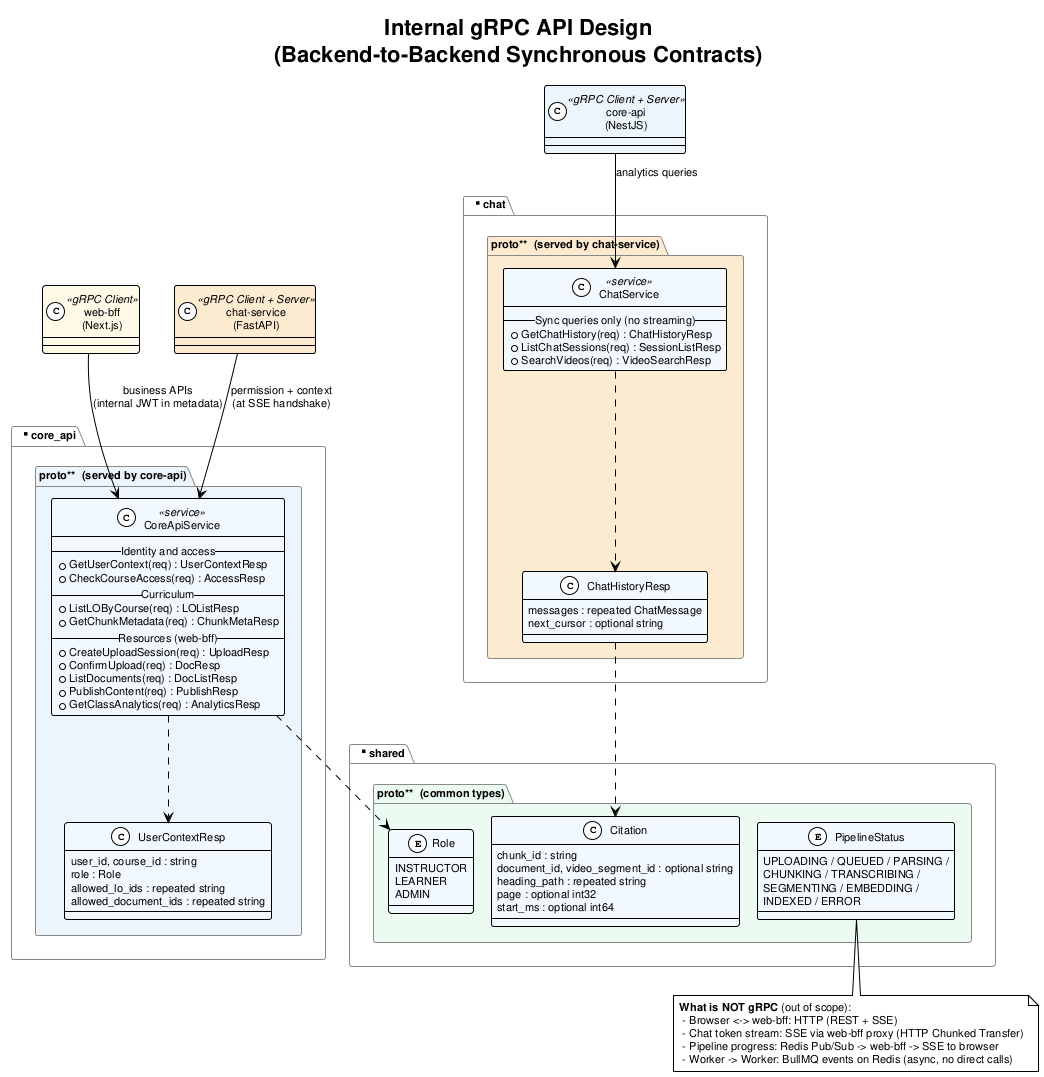
\includegraphics[width=0.95\textwidth]{diagrams/grpc_service_design.png}
    \caption{Internal gRPC API design.}
    \label{fig:grpc-design-lvtn}
\end{figure}

The body keeps only the service boundary needed to understand the
architecture. Full proto-style message definitions and channel rules are
provided in Appendix~\ref{appendix:grpc-proto-details}.

\begin{table}[H]
    \centering
    \caption{Internal service contracts and transport ports.}
    \label{tab:grpc-service-summary}
    \begin{tabular}{|p{3.2cm}|p{2.6cm}|p{7.2cm}|}
        \hline
        \textbf{Boundary} & \textbf{Port} & \textbf{Purpose} \\
        \hline
        Browser $\leftrightarrow$ \texttt{web-bff}
            & HTTPS 443 / dev 3000
            & REST pages, role-based routing, SSE forwarding for chat tokens
              and pipeline progress. \\
        \hline
        \texttt{web-bff} $\to$ \texttt{CoreApiService}
            & gRPC 50051
            & Resource CRUD, upload sessions, review/publish actions, and
              user/course context resolution. \\
        \hline
        \texttt{core-api} $\leftrightarrow$ \texttt{ChatService}
            & gRPC 50052
            & Chat history, audit queries, video search metadata, and
              permission-checked retrieval context. \\
        \hline
        Workers $\leftrightarrow$ event broker
            & Redis 6379
            & BullMQ queues and Pub/Sub progress events for asynchronous
              document, video, and enrichment jobs. \\
        \hline
    \end{tabular}
\end{table}

\subsection{Event-driven Processing}

A stateless event-driven architecture is built on Redis/BullMQ to remove
temporal coupling between complex business components. When a business
event occurs, it is published to trigger the next processing steps:

\begin{itemize}
    \item \textbf{Main events in the system:}
    \begin{itemize}
        \item \texttt{DocumentUploaded}: published by \texttt{core-api}
              after a document file is uploaded successfully, triggering
              text extraction by \texttt{document-worker}.
        \item \texttt{DocumentParsed}: published by
              \texttt{document-worker} to signal that text has been split
              into chunks and persisted successfully in PostgreSQL.
        \item \texttt{TranscriptReady}: published by \texttt{video-worker}
              (Go) after transcript extraction and clip segmentation,
              signaling \texttt{document-worker} to index the transcript.
        \item \texttt{TextIndexed}: published by \texttt{document-worker}
              after document chunks have been upserted to Qdrant and the
              corresponding \texttt{Chunk} nodes plus \texttt{SUPPORTS}
              relationships have been projected into Neo4j. This event
              marks data as ready for downstream pipelines such as
              Micro-Content Generation or Quiz Generation; it is not a
              direct content-generation step in the document pipeline.
        \item \texttt{VideoIndexed}: the corresponding boundary event for
              the video pipeline, published after transcript segments
              have been upserted to Qdrant and projected into Neo4j.
              Downstream consumers (Video Search, Micro-Content) treat
              \texttt{VideoIndexed} the same way as \texttt{TextIndexed}
              but with a different payload (\texttt{video\_id} and
              \texttt{segment\_id} instead of \texttt{document\_id} and
              \texttt{chunk\_id}).
        \item \texttt{ContentGenerationRequested}: published when an
              instructor requests lesson-card or quiz generation for a
              specific content scope, triggering \texttt{enrichment-worker}.
        \item \texttt{ContentDraftGenerated}: published after a card or
              quiz draft has been validated and stored in PostgreSQL with
              \texttt{GENERATED\_DRAFT}.
        \item \texttt{CardPublishedEvent}/\texttt{QuizPublishedEvent}:
              written to \texttt{outbox\_events} in the same transaction
              as publish, then used to synchronize Neo4j.
    \end{itemize}
    \item \textbf{Fault tolerance:} BullMQ uses Exponential Backoff Retry
          (up to 3 retries with increasing delay) for jobs that fail due
          to external API rate limits, and automatically moves raw-text
          format errors to the Dead Letter Queue (DLQ) for manual
          engineering inspection.
\end{itemize}

\subsection{Streaming Architecture}

For direct AI Tutor Chatbot interaction, the system uses one-way
continuous data streaming through Server-Sent Events (SSE) instead of the
heavier bidirectional WebSocket protocol:

\begin{itemize}
    \item \textbf{Technical benefit of SSE:} It perfectly fits the
          one-way token stream of LLM text generation, where the server
          continuously emits generated content to the browser. SSE runs
          over standard HTTP, supports native browser reconnection, has a
          lighter transport mechanism than WebSockets, and passes through
          firewalls/proxies more easily.
    \item \textbf{Token propagation:} When a learner asks a question, the
          request goes to \texttt{chat-service}. The service performs RAG,
          assembles the prompt, and calls Gemini Pro in streaming mode.
          Generated tokens are pushed directly to \texttt{web-bff} through
          Chunked Transfer Encoding. BFF acts as a reverse proxy that
          forwards the text tokens to the learner browser in real time.
\end{itemize}

\section{Security and System Integration Design}

\subsection{LMS Authentication Integration}

The system integrates deeply with Canvas LMS security through LTI 1.3
(Learning Tools Interoperability), built on IMS Security Framework,
OpenID Connect (OIDC), and OAuth 2.0. Authentication and authorization
are designed tightly following the OIDC 3-legged flow to ensure user
identity information is never leaked:

\begin{itemize}
    \item \textbf{OIDC Login Initiation:} When a user clicks the integrated
          system link in Canvas LMS, Canvas sends an HTTP POST/GET request
          to \texttt{/lti/login} of \texttt{web-bff}. The request contains
          parameters such as \texttt{iss}, \texttt{login\_hint},
          \texttt{client\_id}, and \texttt{target\_link\_uri}.
    \item \textbf{OIDC Redirect:} The LTI Integration service validates
          \texttt{client\_id} and \texttt{iss}. It then creates secure
          random values (\texttt{state} and \texttt{nonce}) stored in
          Redis and redirects the user's browser back to the OIDC Auth
          Endpoint of Canvas LMS with these security tokens.
    \item \textbf{Complete LTI Launch (Token Verification):} Canvas LMS
          authenticates the user's login session, then sends an HTTP POST
          containing signed JWT \texttt{id\_token} to
          \texttt{/lti/launch} of \texttt{web-bff}. The system uses the
          public key dynamically configured through Canvas JWKS (JSON Web
          Key Set) to verify the JWT signature. It then validates
          expiration (\texttt{exp}), audience (\texttt{aud}), and nonce
          uniqueness to prevent replay attacks.
    \item \textbf{User and role mapping:} After decoding succeeds, the
          system extracts LTI 1.3 standard claims such as \texttt{sub}
          (LMS User ID), \texttt{roles} (LTI identifiers for Learner or
          Instructor), and class context (\texttt{context.id}). These are
          mapped to the internal database through
          \texttt{lms\_user\_mappings}, and a secure Redis session is
          created.
\end{itemize}

\subsection{Internal Service Authentication (BFF-to-Core JWT)}
\label{subsec:internal-jwt}

Communication between \texttt{web-bff} and business APIs such as
\texttt{core-api} or AI services such as \texttt{chat-service} requires a
strict internal security mechanism while keeping downstream services
stateless:

\begin{itemize}
    \item \textbf{Session-to-Token conversion:} At the outer layer,
          \texttt{web-bff} maintains the user session with a Session ID
          stored in Redis and exchanged through secure
          \texttt{HttpOnly}, \texttt{Secure}, \texttt{SameSite=None}
          cookies, which are required because the tool runs inside a
          Canvas iframe. To avoid making internal backend services query
          Redis repeatedly for session information, the system generates
          short-lived internal JWTs (BFF-to-Core JWT).
    \item \textbf{Internal digital signature:} For each proxied or
          indirect request from BFF into core APIs, \texttt{web-bff} uses
          its locally configured \texttt{Private Key} to sign an internal
          JWT with a very short lifetime, typically 60 seconds.
    \item \textbf{Context propagation:} The internal JWT carries the core
          business context decoded from LTI, including \texttt{user\_id}
          (internal UUID), \texttt{course\_id} (course UUID), and
          \texttt{roles}. Backend services such as \texttt{core-api} or
          \texttt{chat-service} only need BFF's \texttt{Public Key} to
          verify this JWT and perform fine-grained authorization locally,
          without depending on raw session storage.
\end{itemize}

\subsection{API Security}

System API gateways are protected by multiple layers from infrastructure
to application:

\begin{itemize}
    \item \textbf{Transport Layer Security:} Every connection from client
          to \texttt{web-bff} and between services must use HTTPS with TLS
          1.3 (AES-GCM or CHACHA20-POLY1305 cipher suites). HTTP port 80
          only redirects 301 to HTTPS.
    \item \textbf{CORS Policy:} \texttt{web-bff} configures a CORS
          allowlist containing the registered Canvas domain and the
          application domain. All other origins are rejected at the reverse
          proxy layer.
    \item \textbf{CSRF prevention:} The tool runs inside a Canvas
          iframe, so the session cookie must be
          \texttt{SameSite=None; Secure} (Lax/Strict would be dropped on
          cross-site iframe loads). Because \texttt{SameSite=None}
          weakens browser-level CSRF protection, every state-changing
          business API (POST, PUT, PATCH, DELETE) requires an explicit
          \texttt{X-XSRF-TOKEN} header that the frontend reads from a
          separate \emph{double-submit} token cookie (random, per
          session, set on initial render). The LTI Launch itself is a
          cross-site POST and is excluded from CSRF checks because it
          carries an LTI JWT verified against Canvas JWKS.
    \item \textbf{Input Validation:} All API payloads are parsed and
          validated at the adapter layer using schema-based validators
          (\texttt{class-validator} for NestJS and \texttt{Pydantic} for
          FastAPI). Invalid schema values are rejected with HTTP 422
          before entering use cases, reducing injection and runtime errors
          in business logic.
\end{itemize}

\subsection{AI Pipeline Isolation}

LLMs are called through adapters, with three isolation mechanisms:

\begin{itemize}
    \item \textbf{Network egress whitelist:} only
          \texttt{enrichment-worker} and \texttt{chat-service} can access
          LLM provider endpoints. Other runtimes have no outbound route.
    \item \textbf{Tenant isolation:} prompt templates require
          \texttt{\{course\_id\}}, and retrieval is filtered by
          \texttt{course\_id} in Qdrant. Context from different courses is
          never mixed.
    \item \textbf{Cost cap:} every request has a \texttt{max\_tokens}
          ceiling, and each user has daily/monthly quota. Exceeding quota
          returns 429.
\end{itemize}

\subsection{Rate Limiting and Cost Control}

\begin{table}[H]
    \centering
    \caption{Rate limit and quota strategy.}
    \label{tab:rate-limit}
    \begin{tabular}{|p{4cm}|p{4cm}|p{5cm}|}
        \hline
        \textbf{Endpoint/Action} & \textbf{Limit} & \textbf{Scope} \\
        \hline
        Chat message
            & 20/minute, 200/hour
            & Per user \\
        \hline
        Document upload
            & 5/hour, 50/day
            & Per user (instructor) \\
        \hline
        Video upload
            & 2/hour, 10/day
            & Per user (instructor) \\
        \hline
        Quiz attempt
            & 100/hour
            & Per user (learner) \\
        \hline
        LLM token usage
            & 100K tokens/day
            & Per user \\
        \hline
        YouTube API call
            & 100/minute (cache 24h)
            & Whole system \\
        \hline
    \end{tabular}
\end{table}

Rate limiting is designed around a Redis token bucket. LLM token quota
is tracked per user in PostgreSQL table \texttt{user\_llm\_quota} and
reset daily.

\subsection{AI System Security Based on OWASP Top 10 for LLM Applications}
\label{subsec:owasp-llm-summary}

OWASP Top 10 for LLM Applications is a reference for production LLM
risks. Chapter~4 keeps the defense summary in Table~\ref{tab:owasp-llm-summary};
the detailed risk and mitigation discussion is moved to
Appendix~\ref{appendix:owasp-llm-details}.

\begin{table}[H]
    \centering
    \caption{Summary of OWASP LLM risk mitigations.}
    \label{tab:owasp-llm-summary}
    \begin{tabularx}{\textwidth}{|p{3.4cm}|X|}
        \hline
        \textbf{Risk area} & \textbf{Main mitigation in this system} \\
        \hline
        Prompt Injection
            & Separate system/user prompts, delimit user input, detect
              injection patterns, and restrict answers to approved context. \\
        \hline
        Sensitive Data Leakage
            & Enforce \texttt{course\_id} retrieval filters, redact PII before
              indexing, restrict log access, and keep quiz answer keys out of
              chat context. \\
        \hline
        Unsafe Output Handling
            & Validate structured LLM output with JSON schemas, sanitize
              rendered content, and never execute generated text. \\
        \hline
        Malicious Document Upload
            & Whitelist file types, scan/sandbox parsing, apply time and memory
              limits, and keep parser dependencies patched. \\
        \hline
        Vector Database Poisoning
            & Allow instructor-only uploads, moderate suspicious chunks, audit
              vector writes, and delete vectors through the outbox cleanup
              saga. \\
        \hline
        Excessive Agency
            & Give the LLM no destructive tools; restrict tool use to validated,
              audited, read-only retrieval such as video search. \\
        \hline
        Overreliance on AI Output
            & Require Human-in-the-Loop review, show source citations, and avoid
              automatic publishing. \\
        \hline
        Insecure Plugin / Tool Design
            & Validate tool input schemas, sanitize tool output, whitelist
              external URLs, and apply tool-level timeouts/rate limits. \\
        \hline
        Training Data Poisoning
            & Not applicable to the MVP because no fine-tuning is used; future
              fine-tuning requires dataset audit and regression evaluation. \\
        \hline
        Supply Chain Vulnerabilities
            & Pin dependencies, scan packages and images, use trusted base
              images, and prefer self-hosted embeddings for core retrieval. \\
        \hline
    \end{tabularx}
\end{table}

\section{Interface Design}
\label{sec:interface-design}

\subsection{UI/UX Design Philosophy}

\subsubsection*{a. Calm UI/UX}

The UI follows the \textbf{Calm UI} philosophy: static, clean, and low on
effects. The goal is to help learners focus on content without being
distracted by unnecessary animations or notifications.

\begin{itemize}
    \item White/light-gray background, minimal accent color.
    \item Clear typography (system font stack), high contrast.
    \item Animations only for direct feedback (loading, success, error).
    \item No advertising pop-ups and no marketing nudges.
\end{itemize}

\subsubsection*{b. Minimal Distraction Learning}

In learning screens (card view, video learning, chatbot), the UI removes
irrelevant elements:

\begin{itemize}
    \item Sidebar and header collapse during learning.
    \item Notifications are deferred to a separate notification center.
    \item ``Focus mode'': only content and basic controls are visible.
\end{itemize}

\subsubsection*{c. Progressive Disclosure}

Information is revealed gradually when needed:

\begin{itemize}
    \item Cards show key insight first; bullet details expand on tap.
    \item Quiz feedback shows right/wrong immediately; detailed
          explanation opens on tap.
    \item Chat citations show links first; full chunk content opens on tap.
\end{itemize}

Detailed sitemap and screen-level descriptions are provided in
Appendix~\ref{appendix:ui-details}. The representative wireframe below
keeps one concrete UX artifact in the main chapter because the
Human-in-the-Loop review interface is the highest-risk decision point
before AI-generated content reaches learners.

\subsection{Representative Wireframe: Instructor Review}
\label{subsec:representative-wireframe}

\begin{figure}[H]
    \centering
    \fbox{%
    \begin{minipage}{0.9\textwidth}
        \vspace{0.2cm}
        \textbf{Review Inbox} \hfill Course selector \quad Filter: Draft / Reviewing / Changes requested

        \vspace{0.25cm}
        \begin{tabular}{|p{3.2cm}|p{8.9cm}|}
            \hline
            Queue & Selected item preview \\
            \hline
            Card draft 01 \newline
            Quiz item 02 \newline
            Card draft 03
                & Title, generated card or quiz content, source chunk preview,
                  citation link, and AI-generated badge. \\
            \hline
            Actions
                & Approve \quad Edit \quad Reject \quad Request regeneration
                  \quad View audit trail. \\
            \hline
        \end{tabular}

        \vspace{0.2cm}
        Bottom area: diff panel for edits and timeline of reviewer actions.
        \vspace{0.2cm}
    \end{minipage}}
    \caption{Representative wireframe of the instructor review interface.}
    \label{fig:wireframe-review-interface}
\end{figure}

\section{Sequence Diagram: LTI Launch}
\label{sec:lti-launch-sequence}

Only the LTI Launch sequence is kept in this chapter because it is the
single integration point with Canvas and the foundation of every
downstream authorization check; understanding it is required to follow
the security design in
Section~\ref{subsec:internal-jwt} and the gRPC API boundary in
Section~\ref{subsec:grpc-internal-apis}. The remaining sequence
diagrams (document upload, video upload, AI Tutor chatbot, quiz
generation, curriculum ingestion) follow the same canonical patterns
described in the AI Pipeline section above and are provided in full in
Appendix~\ref{appendix:sequence-diagrams}.

\begin{figure}[H]
    \centering
    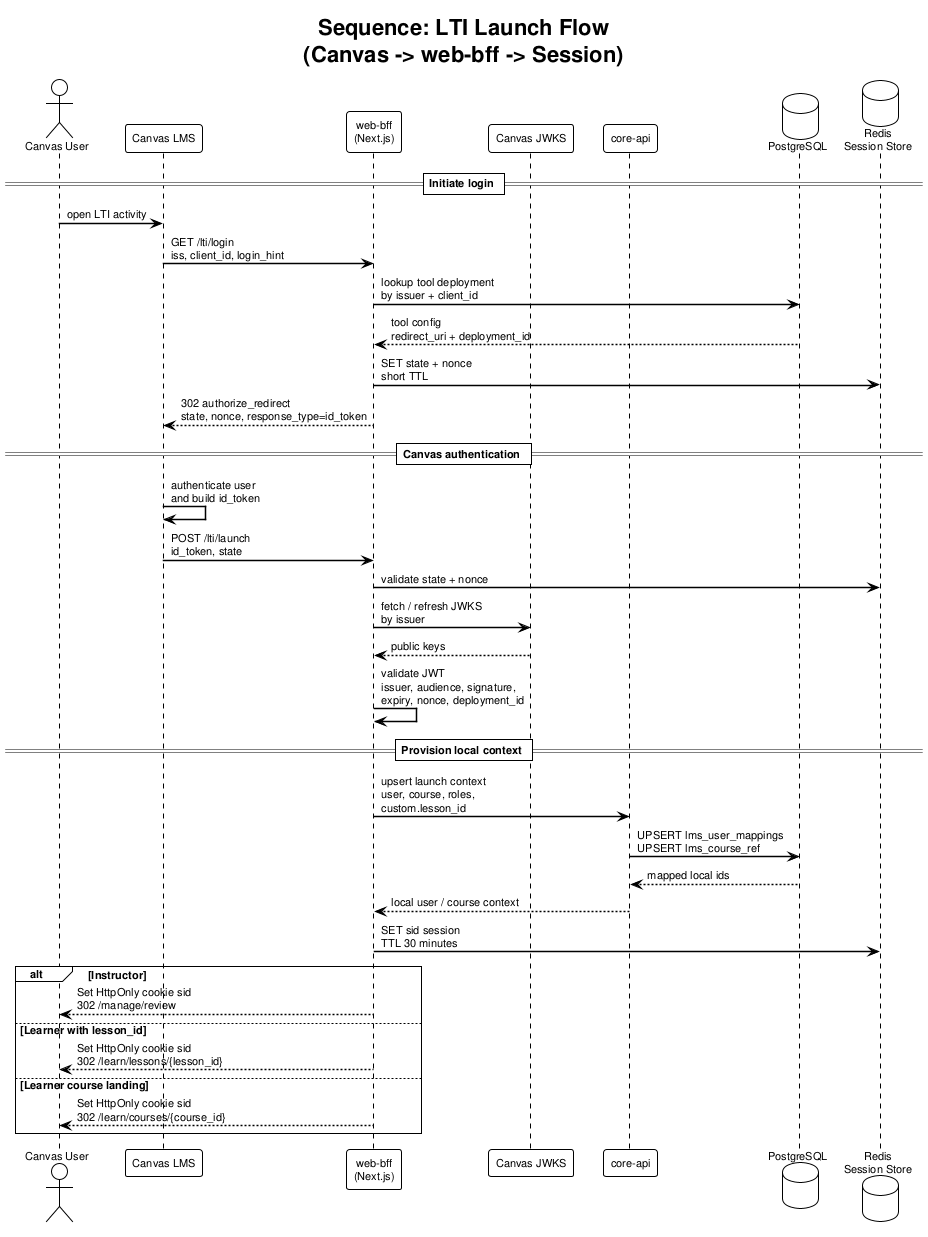
\includegraphics[width=0.95\textwidth]{diagrams/seq_lti_launch.png}
    \caption{Sequence diagram for LTI launch from Canvas into the system.}
    \label{fig:seq-lti-launch}
\end{figure}

\begin{enumerate}
    \item Learner logs into Canvas and opens an activity containing the
          LTI tool.
    \item Canvas $\to$ \texttt{web-bff} \texttt{/lti/login} with
          \texttt{iss}, \texttt{client\_id}, \texttt{login\_hint}.
    \item \texttt{web-bff}: lookup tool config, redirect to Canvas
          \texttt{/api/lti/authorize\_redirect} with
          \texttt{state}, \texttt{nonce}, \texttt{response\_type=id\_token}.
    \item Canvas authenticates the user, generates \texttt{id\_token} JWT,
          and form POSTs to \texttt{web-bff} \texttt{/lti/launch}.
    \item \texttt{web-bff}: validate JWT (issuer, audience, signature
          through Canvas JWKS, exp, nonce).
    \item Extract claims: \texttt{sub}, \texttt{context.id},
          \texttt{context.title}, \texttt{roles},
          \texttt{custom.lesson\_id} (if Deep Linking exists).
    \item \texttt{web-bff} $\to$ \texttt{core-api}: UPSERT
          \texttt{lms\_user\_mappings}, \texttt{lms\_course\_ref}.
    \item Set Redis session with TTL 30 minutes.
    \item Cookie HttpOnly \texttt{sid}, 302 redirect:
        \begin{itemize}
            \item Instructor: \texttt{/manage/review}.
            \item Student with \texttt{custom.lesson\_id}:
                  \texttt{/learn/lessons/\{lesson\_id\}}.
            \item Student without a specific context:
                  \texttt{/learn/courses/\{course\_id\}}.
        \end{itemize}
\end{enumerate}

\section{Class Diagram}

The class diagram represents the main domain entities and their
relationships, split into two bounded contexts to keep each figure
readable. Only \emph{Content Authoring} is included here because it
carries the \texttt{Lesson} aggregate -- the unit of LTI Deep Linking
and the most architecturally load-bearing entity. The
\emph{Curriculum} bounded context (Course, Chapter, LearningOutcome,
Assessment, ChunkLOMapping) is provided in
Appendix~\ref{appendix:class-diagrams}. Field names mirror the
PostgreSQL schema in Appendix~\ref{appendix:db-schema}.

\subsection{Bounded Context: Content Authoring}

This context owns raw materials (documents and videos), derived chunks
and transcript segments, and the AI-generated artifacts grouped under a
\texttt{Lesson} aggregate. The \texttt{Lesson} entity is the unit of
LTI Deep Linking: its \texttt{lesson\_id} is surfaced in
\texttt{custom.lesson\_id} on launch and in the URL
\texttt{/learn/lessons/\{id\}}. Each lesson is uniquely scoped to one
Learning Outcome (\texttt{UNIQUE(course\_id, lo\_id)}) and acts as the
publication boundary for its cards and quiz items.

\begin{figure}[H]
    \centering
    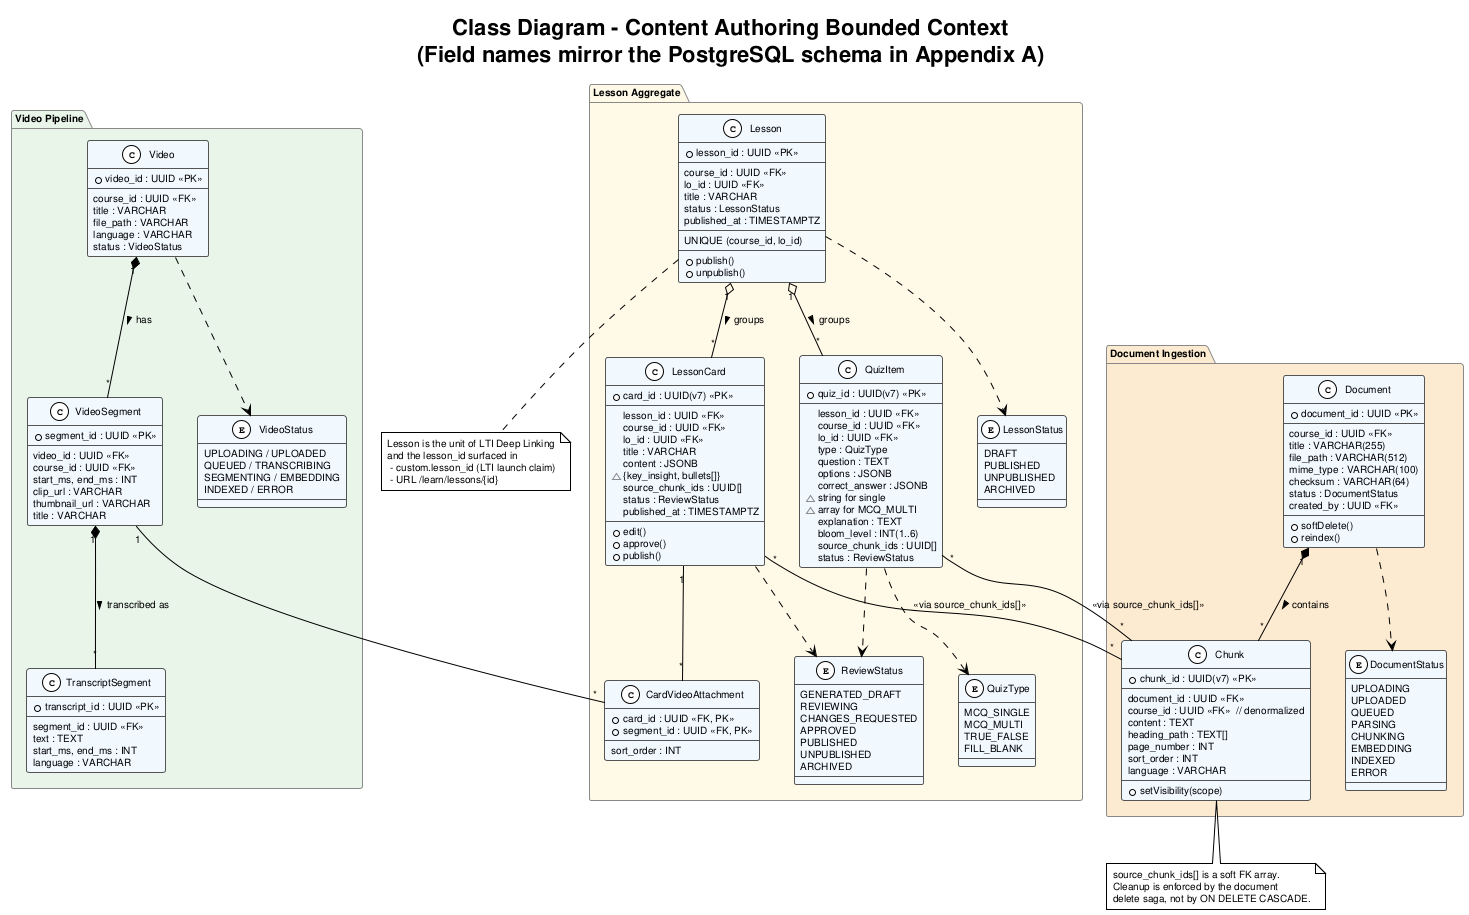
\includegraphics[width=\textwidth,height=0.88\textheight,keepaspectratio]{diagrams/class_diagram_content_authoring.png}
    \caption{Class diagram of the Content Authoring bounded context.}
    \label{fig:class-content-authoring}
\end{figure}

The dashed many-to-many edges from \texttt{LessonCard} and
\texttt{QuizItem} to \texttt{Chunk} are realized through the
\texttt{source\_chunk\_ids[]} array column rather than a join table; the
referential integrity is preserved by the document delete saga
(Appendix~\ref{appendix:delete-saga}) rather than by
\texttt{ON DELETE CASCADE}.

\subsection{Port Interfaces (Hexagonal Domain)}

The domain layer exposes the following Ports; each Port has one or
more Adapters implemented with concrete technologies (see the Layered
Architecture subsection and the Adapter design section):

\begin{itemize}
    \item \texttt{IParser}, \texttt{IChunker}, \texttt{IEmbeddingModel}
    \item \texttt{IVectorStore}, \texttt{IMetadataStore},
          \texttt{IGraphStore}
    \item \texttt{IObjectStorage}, \texttt{ILLMClient}
    \item \texttt{ICurriculumExtractor}, \texttt{IChunkLOMapper}
    \item \texttt{IVideoSearchClient}, \texttt{IMcpYouTubeTool}
\end{itemize}

\section{State Machine Design}
\label{sec:state-machine-design}

The system uses three independent state machines that cover three
different concerns: the business state of document/video processing
(Section~\ref{subsec:document-pipeline-state}), the broker-level state
of asynchronous BullMQ jobs
(Appendix~\ref{appendix:state-async-job}), and the review lifecycle of
generated cards/quizzes
(Appendix~\ref{appendix:state-content-review}). Keeping these state
machines separate prevents business state from being coupled to retry
mechanics or content-review workflow. Only the user-visible business
state machine is shown in this chapter; the other two are placed in
Appendix~\ref{appendix:state-machines} because they belong to
operational and review concerns rather than the main design
narrative.

\subsection{Document and Video Pipeline State}
\label{subsec:document-pipeline-state}

\begin{figure}[H]
    \centering
    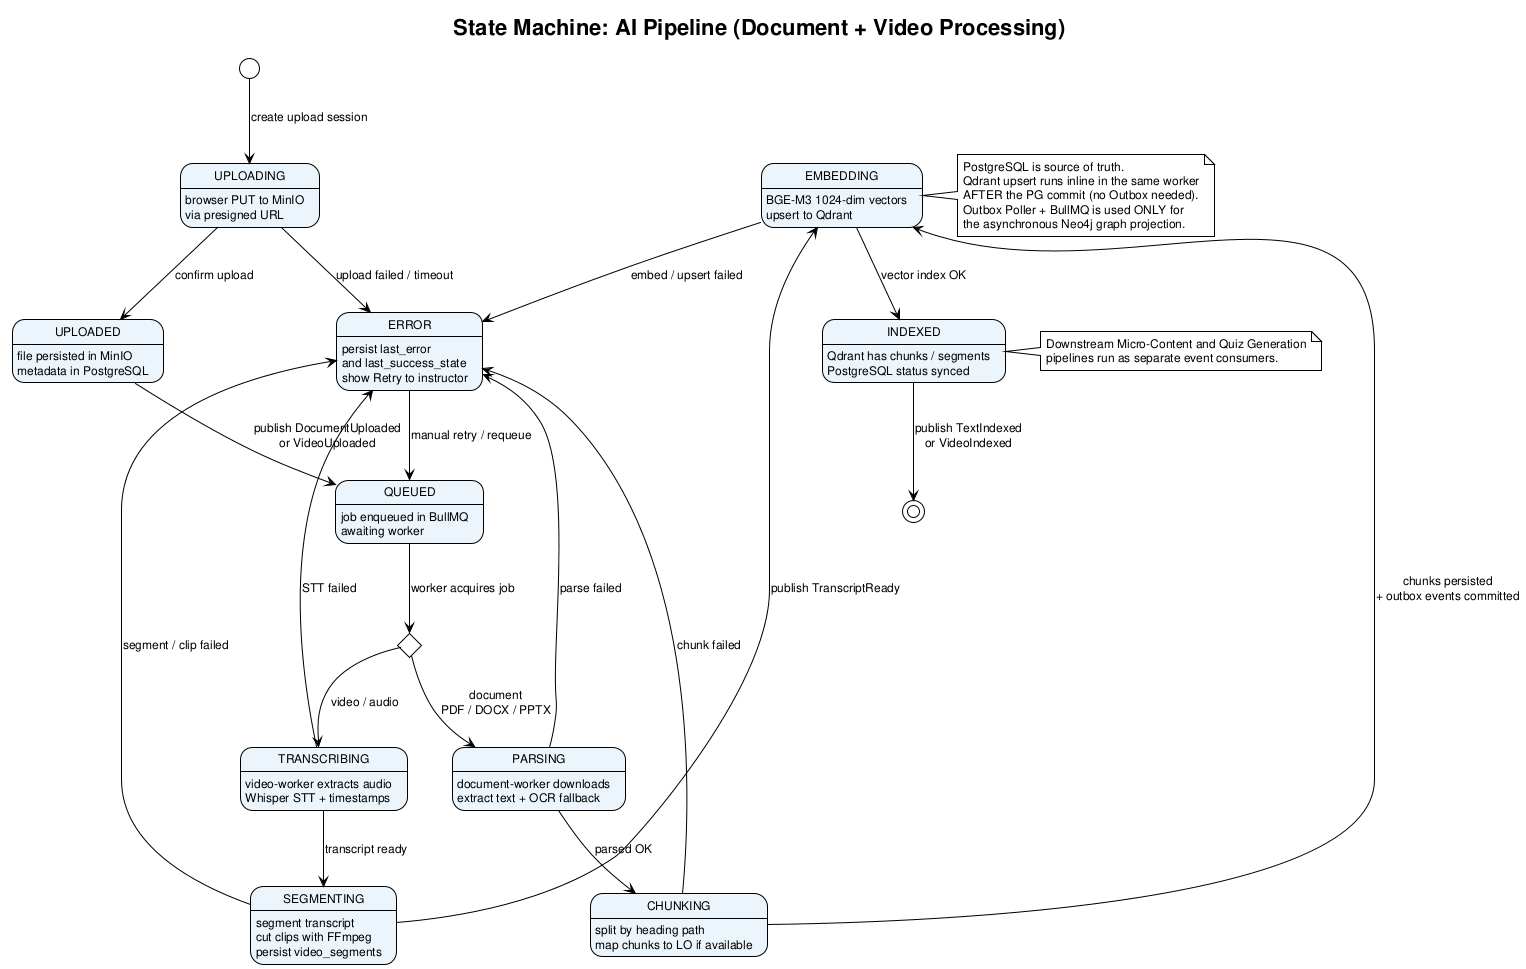
\includegraphics[width=0.85\textwidth]{diagrams/state_machine_pipeline.png}
    \caption{State machine of the document/video processing pipeline.}
    \label{fig:state-machine}
\end{figure}

After the upload session, the pipeline branches into two parallel
processing paths depending on input type: documents go through
\texttt{PARSING} $\to$ \texttt{CHUNKING}, while videos go through
\texttt{TRANSCRIBING} $\to$ \texttt{SEGMENTING}. Both branches converge
at \texttt{EMBEDDING} and end at \texttt{INDEXED}.

\begin{table}[H]
    \centering
    \caption{States of the document/video pipeline.}
    \label{tab:doc-states}
    \begin{tabular}{|p{3.6cm}|p{2cm}|p{7.5cm}|}
        \hline
        \textbf{State} & \textbf{Branch} & \textbf{Meaning} \\
        \hline
        \texttt{UPLOADING}
            & Both
            & Browser is uploading to MinIO via presigned URL. \\
        \hline
        \texttt{UPLOADED}
            & Both
            & Upload completed, waiting for confirmation. \\
        \hline
        \texttt{QUEUED}
            & Both
            & Event published to BullMQ, waiting for worker. \\
        \hline
        \texttt{PARSING}
            & Document
            & \texttt{document-worker} extracts text (OCR fallback if
              needed). \\
        \hline
        \texttt{CHUNKING}
            & Document
            & Text is split into chunks by heading path; LO mapping is
              applied. \\
        \hline
        \texttt{TRANSCRIBING}
            & Video
            & \texttt{video-worker} extracts audio (FFmpeg) and runs
              Whisper STT. \\
        \hline
        \texttt{SEGMENTING}
            & Video
            & Transcript is segmented; clips are cut and stored in
              MinIO. \\
        \hline
        \texttt{EMBEDDING}
            & Both
            & BGE-M3 generates 1024-dim vectors for chunks or transcript
              segments. \\
        \hline
        \texttt{INDEXED}
            & Both
            & Vectors are upserted to Qdrant and the content is
              searchable. \\
        \hline
        \texttt{ERROR}
            & Both
            & Pipeline failed; \texttt{last\_error} and
              \texttt{last\_success\_state} are persisted so the
              instructor can request a manual retry. \\
        \hline
    \end{tabular}
\end{table}

Any failed stage transitions to \texttt{ERROR}; from there a manual
retry returns the job to \texttt{QUEUED}. Content-generation states
such as \texttt{GENERATED\_DRAFT} are intentionally not part of this
pipeline; they belong to a separate review lifecycle.

\subsection{Supporting State Machine Designs}
\label{subsec:other-state-machines}

Two additional state machines support the operational and review
lifecycle of the system, but they are not required to follow the main
design narrative. Their full diagrams and state tables are provided in
Appendix~\ref{appendix:state-machines}:

\begin{itemize}
    \item \textbf{Asynchronous Job State (BullMQ)} -- broker-level
          retry/dead-letter semantics, intentionally decoupled from
          business state
          (Appendix~\ref{appendix:state-async-job}).
    \item \textbf{Content Review State (LessonCard / QuizItem)} --
          Human-in-the-Loop lifecycle
          \texttt{GENERATED\_DRAFT} $\to$ \texttt{REVIEWING} $\to$
          \texttt{APPROVED} $\to$ \texttt{PUBLISHED}
          (Appendix~\ref{appendix:state-content-review}).
\end{itemize}

\section{Observability and Monitoring Design}
\label{sec:observability-monitoring-design}

Observability follows three standard pillars, with AI cost monitoring as
a fourth project-specific concern. Detailed log fields, metric names,
trace spans, and alert examples are provided in
Appendix~\ref{appendix:observability-details}.

\begin{table}[H]
    \centering
    \caption{Observability overview.}
    \label{tab:observability-overview}
    \begin{tabular}{|p{3.2cm}|p{10.2cm}|}
        \hline
        \textbf{Concern} & \textbf{Design summary} \\
        \hline
        Structured logs
            & Every runtime emits JSON logs with service name and trace
              correlation, aggregated into Loki or Elasticsearch. \\
        \hline
        Metrics
            & Prometheus scrapes service, worker, business, and system metrics;
              Grafana shows latency, throughput, error rate, saturation, and
              queue depth. \\
        \hline
        Distributed traces
            & OpenTelemetry propagates \texttt{traceparent} through HTTP, gRPC,
              SQL, vector search, graph access, storage, and LLM calls. \\
        \hline
        AI cost
            & Token usage, model/provider, user, course, and use-case
              dimensions are tracked to support quota enforcement and
              cost-spike alerts. \\
        \hline
    \end{tabular}
\end{table}

\section{System Deployment Design}
\label{sec:system-deployment-design}

\begin{figure}[H]
    \centering
    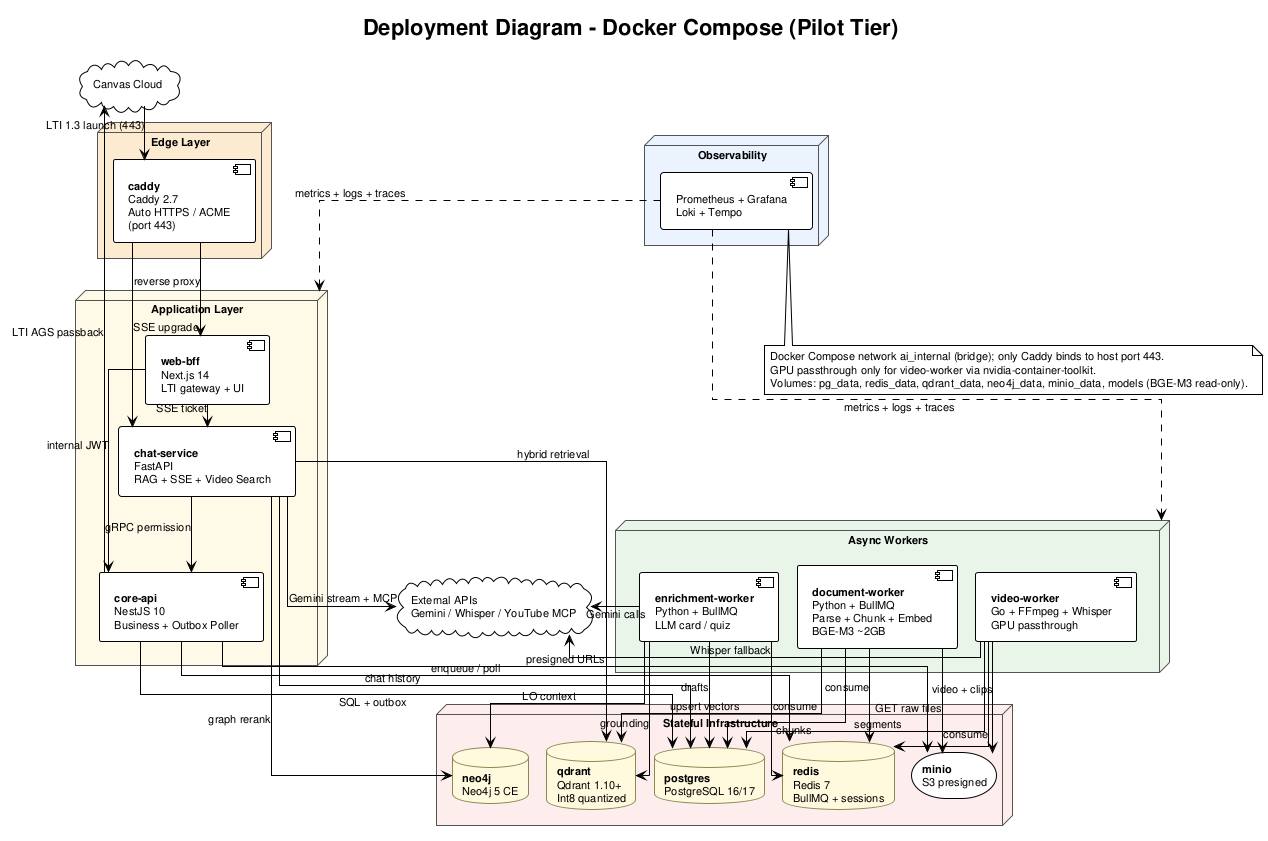
\includegraphics[width=0.95\textwidth]{diagrams/deployment_diagram.png}
    \caption{Deployment topology.}
    \label{fig:deployment}
\end{figure}

The deployment model uses Docker Compose with a main \texttt{ai-system}
stack and an optional LMS stack for self-hosted demo environments. In
production, Canvas is normally external; only the reverse proxy and
\texttt{web-bff} need public HTTPS exposure for OIDC/LTI launch, while
workers, databases, vector search, graph storage, object storage, and
observability components stay on internal networks. Compose service,
network, and volume details are kept in
Appendix~\ref{appendix:deployment-details}.

\subsection{CI/CD Direction}

The CI/CD pipeline contains four stages:

\begin{enumerate}
    \item \textbf{Build:}
        \begin{itemize}
            \item Lint (ruff/eslint), type check (mypy/tsc).
            \item Unit test (pytest, jest) with Mock Adapter.
            \item Build Docker image for each runtime, tagged by commit
                  SHA.
        \end{itemize}
    \item \textbf{Integration test:}
        \begin{itemize}
            \item Docker Compose up with testcontainers
                  Postgres/Redis/Qdrant.
            \item Run integration tests that call real RPC/HTTP paths
                  between services.
        \end{itemize}
    \item \textbf{Deploy staging:}
        \begin{itemize}
            \item Push image to registry.
            \item SSH deploy to staging server, \texttt{docker compose
                  pull}, \texttt{docker compose up -d}.
            \item Smoke test health endpoints.
        \end{itemize}
    \item \textbf{Deploy production:} after manual approval.
\end{enumerate}

Tooling: GitHub Actions or GitLab CI.

\subsection{Scaling Strategy}

\textbf{Vertical scaling (single-node):} increase CPU/RAM for the heaviest
containers (\texttt{document-worker}, \texttt{enrichment-worker},
\texttt{video-worker}). This is enough for the project project.

\textbf{Horizontal scaling (multi-node, production):}
\begin{itemize}
    \item \texttt{web-bff}, \texttt{core-api}, \texttt{chat-service}:
          stateless, linearly scalable by replica.
    \item \texttt{document-worker}, \texttt{enrichment-worker}: scale
          replicas by queue depth; each replica consumes from Redis in
          parallel.
    \item \texttt{video-worker}: scale replicas by pending video count.
    \item Postgres: read replicas for query-heavy workloads (analytics
          dashboard).
    \item Qdrant: cluster mode with shard by \texttt{course\_id} when
          needed.
    \item Neo4j: read replica or Fabric for heavy queries.
\end{itemize}

\textbf{Expected bottleneck:} LLM API rate limits. Mitigation uses request
batching, prompt caching, and fallback models (Gemini Flash when Pro quota
is exhausted).

\section{Chapter Summary}

This chapter has presented the complete system design at the architectural
level:

\begin{itemize}
    \item \textbf{Multi-runtime architecture} with six physical runtimes
          (\texttt{web-bff}, \texttt{core-api}, \texttt{chat-service},
          \texttt{document-worker}, \texttt{enrichment-worker},
          \texttt{video-worker}) and nine logical services distributed
          across those runtimes, clearly separating UI, business logic,
          realtime AI, CPU-bound AI batch work, I/O-bound AI batch work,
          and media processing.
    \item \textbf{Canvas LMS integration} through LTI 1.3 / OIDC, using an
          AI Extension Layer rather than building a custom LMS.
    \item \textbf{Nine logical services}, including the Video Search module
          inside \texttt{chat-service} (searching uploaded videos through
          Qdrant and YouTube through MCP), which is a distinguishing point
          of the system.
    \item \textbf{Six AI pipelines} (document, video, RAG,
          Micro-Content, quiz, review/publish) orchestrated through
          Redis + BullMQ event-driven processing.
    \item \textbf{Five data stores} (Postgres, Qdrant, Neo4j, Redis,
          MinIO), with PostgreSQL as the source of truth (31 core tables
          plus 2 concept-tag extension tables);
          other stores are derived and synchronized through the outbox
          pattern.
    \item \textbf{Security} follows OWASP Top 10 for LLM Applications with
          10 concrete mitigations from prompt injection to supply chain.
    \item \textbf{UI/UX} follows Calm UI, Minimal Distraction,
          Progressive Disclosure, and Mobile-first principles.
    \item \textbf{Observability} covers the three pillars: structured
          logging, Prometheus metrics, and OpenTelemetry distributed
          tracing, with separate AI cost monitoring.
    \item \textbf{Deployment} uses Docker Compose for the project,
          packaged as three layered files (base, dev override, GPU override).
\end{itemize}

This design allows \textbf{parallel development} among team members thanks
to clear service boundaries, \textbf{flexible replacement} of adapters
(LLM provider, vector store, LMS) through Hexagonal Architecture, and
\textbf{independent scaling} of each pipeline as load grows. The next
chapter presents implementation details, including code structure,
selected technologies, and technical decisions during development.
